Effects on the \detdeta measurements from a large set of systematic variations were tested to determine the overall systematic uncertainties on the measurements. 
The individual items for each systematic source are listed as following:
\begin{itemize}
    \item Calorimeter calibration 
    \item Intermittant hot tower masking
    \item Calorimeter hadronic response modeling
    \item MC reweighting
    \item Zero suppression application
    \item Detector acceptance
    \item Global uncertainties (z-vertex, \Npart determination)
\end{itemize}

\subsection{Calorimeter Calibrations}

Systematic uncertainties were included to account for the uncertainty for the absolute calibration of each of the three calorimeter layers (EMCal, IHCal and OHCal). 
The EMCal systematic uncertainties account for the statistical uncertainty on the $\pi^{0}$ mass peak used for the absolute energy scale calibration, the tower-by-tower statistical uncertainty on the Tower Slope Calibration factors used for the gain balancing relative calibrations within a $\eta$ slice of the calorimeter, and for data and MC differences in the extracted $\pi^{0}$ mass peak, including resolution difference studied by varying the MC smearing and seeing the effect on the predicted $\pi^{0}$ mass value~\cite{EMCal_calib_internal_note}.
The total effect of these calibration systematics on the EMCal \detdeta is 2.6\% over all centrality bins studied in this measurement. 
The vast majority of this uncertainty comes from the variation due to data and MC differences in the $\pi^{0}$ mass peak width.

Three systematic uncertainties were also included to account for the uncertainty in each of the HCal's absolute EM scale calibration~\cite{HCal_calib_internal_note}. 
To find tower by tower calibration factors from cosmic muons, the ratio of MPV, or most probable value, is taken in MC/data; 
a gamma function fit is used in the nominal calibration procedure to extract the MPV. 
The HCal's absolute EM scale calibration systematic uncertainties are determined from both the statistical and systematic errors in the fitting of these cosmics MIP distributions and data to MC comparisons of the HCal transverse energy.
The total effect of these calibration systematics on the HCal \detdeta is 2.7\% over all centrality bins studied in this measurement. 

Finally, the total effect of these calibration systematics on the full calorimeter \detdeta measurement is 2.1\%.
Contributions from each of the calibration variations to the \detdeta measurements are included in detail in Table \ref{table:SystUncertainties}.

\subsection{Intermittent Hot Tower Masking}
\label{hot_tower_syst}

To study the effect of changing calorimeter acceptance from masking towers with bad quality factors on the event-by-event level, the dataset was split into 1\% centrality intervals.
For each centrality interval, the variation in the $\detdeta$ measurement was found between either excluding events with intermittent hot towers or including these events with intermittent hot towers but masking the bad channel(s) thereby slightly changing the calorimeter acceptance. 
The smallest centrality intervals possible of 1\% were used in this study since the rate of intermittent hot towers is slightly centrality dependent due to occupancy differences in central versus peripheral events.
These steps were taken to make as direct a comparison as possible of the effects of only the small changes in calorimeter acceptance (on the level of 1 tower) on the $\detdeta$ measurement. 
This variation was found to be negligible for all measurements and all centrality intervals in the analysis. 

\subsection{Calorimeter Hadronic Response Modeling}

Data to MC comparisons of the $\langle E_{e} \rangle/\langle E_{\pi} \rangle$ response from the sPHENIX test beam paper were used to estimate the uncertainty in the calorimeter hadronic response~\cite{emcal_hcal_beamtest}; 
this comparison is included in Figure~\ref{fig:testbeam_eoverpi}. 
For these data to MC comparisons, the \geant simulation physics lists and Birk's constants were varied to determine a range of possible hadronic responses and compared with test beam data collected by the sPHENIX prototypes. 
The full range of possible simulation curves is used in the estimation of the hadronic response uncertainty and this range is estimated to be uniformly distributed across the range of simulation curves resulting in a final hadronic response uncertainty from these test beam data to MC comparisons of 6.8\%. 

The \geant simulation physics lists determine the modeling of shower development in the simulated calorimeters~\cite{geant_physics_list}.
The default \geant simulation physics list recommended for collider physics applications is called "FTFP\_BERT"~\cite{FTFP_BERT_model}, which uses two models at different energy ranges to model hadronic interactions: the Fritiof (FTF) model for high energy interactions (3 GeV to 100 GeV) and the Bertini (BERT) cascade model for low energy interactions (0 GeV to 6 GeV).
An older physics list, "QGSP\_BERT"~\cite{QGSP_BERT_model}, uses the Quark-Gluon String (QGS) model for high energy interactions (12 GeV+), the Fritiof model for intermediated energy interactions (3 GeV to 25 GeV) and the same Bertini cascade model for low energy interactions (0 GeV to 6 GeV).
For overlap regions where two models are used, a model is selected by sampling a probability distribution that scales linearly with energy between 0 and 1 across the overlap region.
In both cases, a "HP" version of the physics list is available which includes high precision neutron modeling for neutrons $< 20$ MeV.

The Birk's constant is used as a tunable parameter used in the Birk's law formula to model the scintillation light yield from energy deposits in scintillator material~\cite{Birks:1951boa}.
Birk's law is as follows:
\begin{equation}
    \frac{dL}{dx} = S\frac{dE/dx}{1+kB(dE/dx)}
\end{equation}
where $L$ is the light yield, $S$ is the scintillation efficiency, $dE/dx$ is the deposited energy per unit length and $kB$ is the Birk's constant. 
The Birk's constant is in theory a material property of the scintillator, for example, for the 
polystyrene-based scintillators used in the sPHENIX HCal, a Birk's constant of 0.008 cm/MeV is typically used.
However, in detector simulations, the Birk's constant is treated as a tunable parameter that is varied to reproduce the calorimeter response to hadrons seen in data that is not accounted for by the models in the \geant physics lists alone.
Therefore, the Birk's constant in practice accounts for both the light quenching which is a material property of the scintillator and any additional discrepancies in the \geant modeling of the shower processes that lead to differences in the calorimeter response between data and simulation.

\begin{figure}
    \centering
    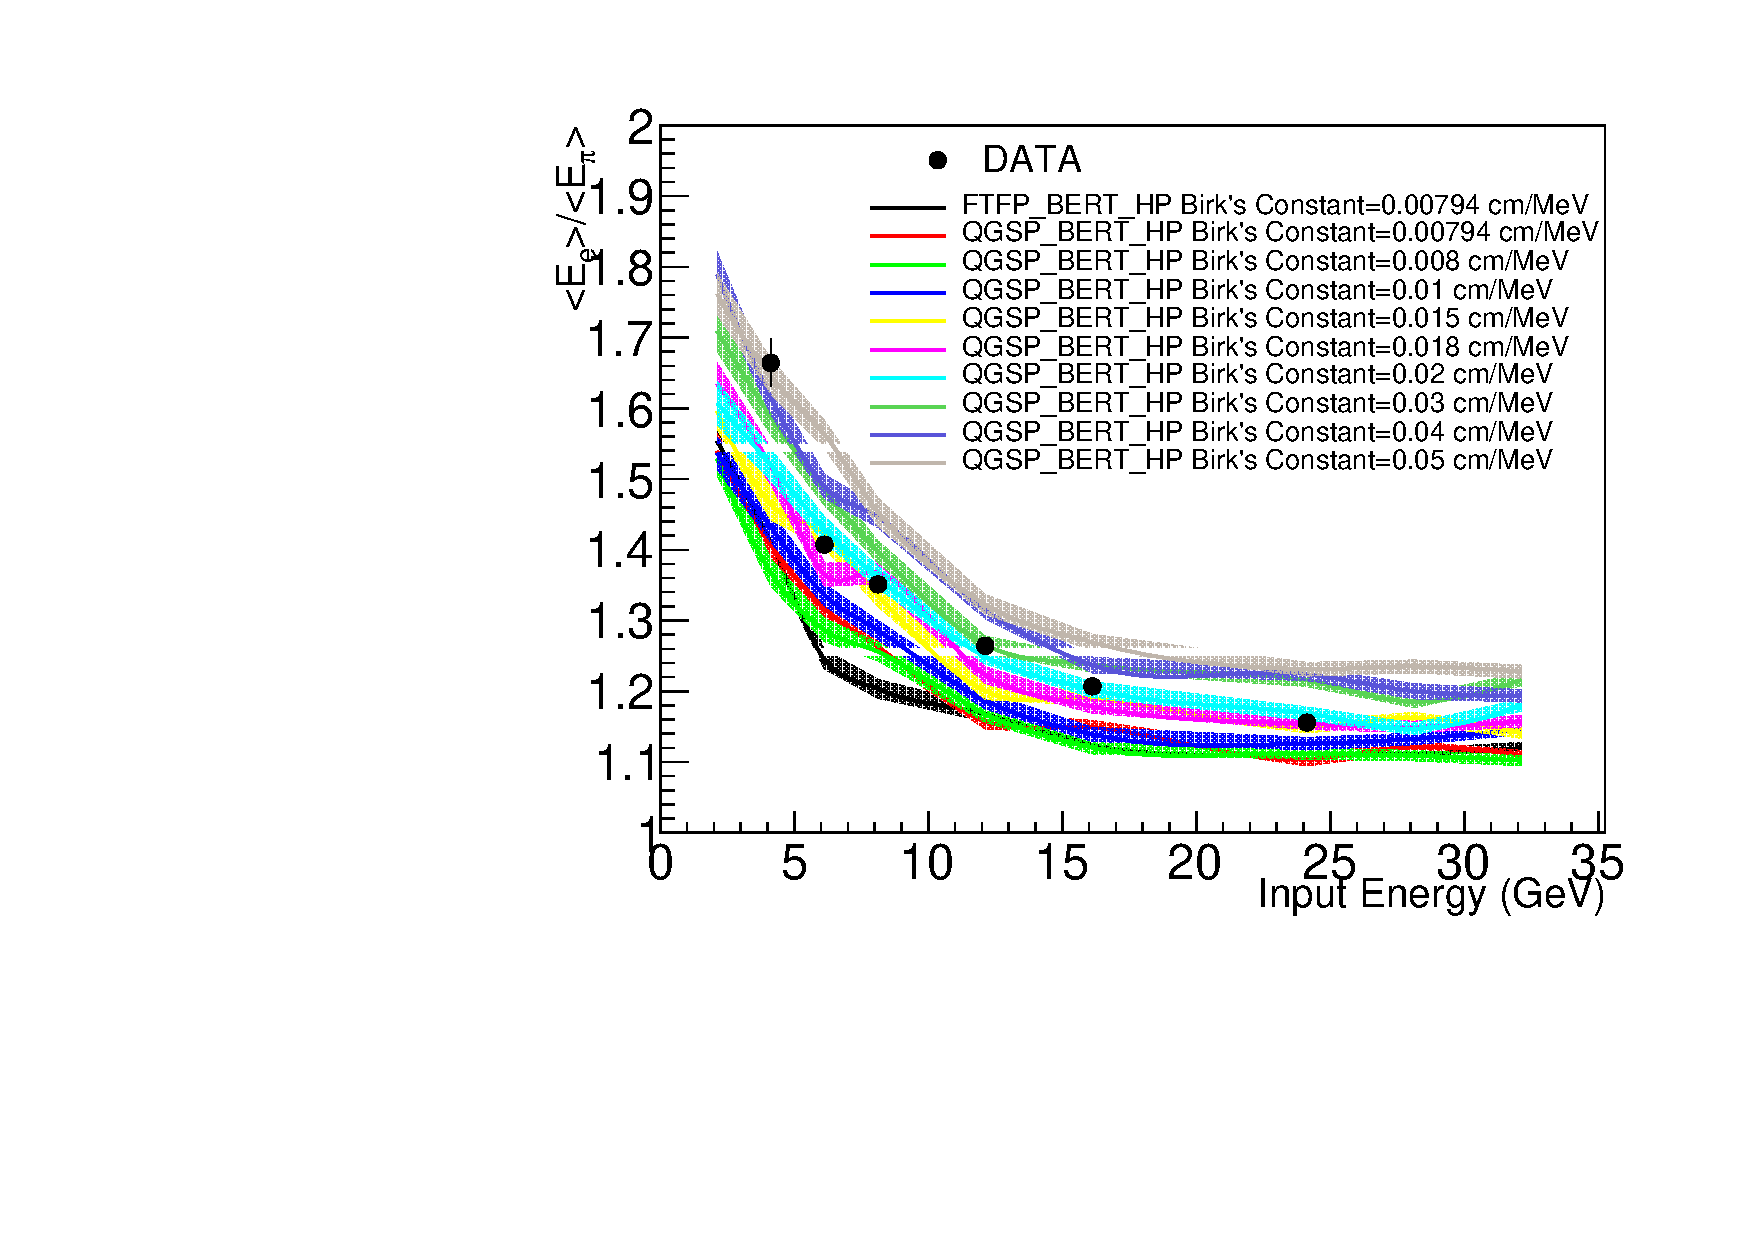
\includegraphics[width=0.8\linewidth]{detdeta/Figures/hadronic_fraction_syst/HCAL_standalone_eoverpi.pdf}
    \caption{HCal $\langle E_{e} \rangle/\langle E_{\pi} \rangle$ response. Test beam data is compared with several different simulation setups by changing physics lists and Birks’ constants. Reproduced from~\cite{emcal_hcal_beamtest}.}
    \label{fig:testbeam_eoverpi}
\end{figure}

This hadronic response uncertainty was then multiplied by the fraction of hadronic energy seen in each of the individual calorimeter layers to determine the hadronic response uncertainty for measurements with each calorimeter configuration (EMCal, HCal, full calorimeter, IHCal-only and OHCal-only).
The fraction of hadronic energy in each of the calorimeter layers was determined from simulation using the same reweighted \epos dataset used to determine our \detdeta correction factors. 
An additional check of hadronic fraction of energy in each calorimeter was done using the reweighted \ampt and \hijing datasets and found to be consistent with the reweighted \epos dataset results.

The hadronic versus EM energy fractions were determined in the sPHENIX \geant simulation for each calorimeter layer via the calorimeter scintillator G4Hits light yield. 
Whether an energy deposit in the calorimeter's scintillator was considered to be EM or hadronic energy was determined by tracing this deposit back to its primary particle and checking the particle type.
Contributions to EM-only energy fraction came from primary $e^{+/-}$, $\gamma$ and $\pi^{0}$ particles, while all other particles contributed to the hadronic energy fraction.
Figure~\ref{fig:hadronic_fraction_syst} shows the event-by-event fraction of hadronic energy seen in each of the calorimeter layers; the average EMCal average hadronic energy fraction is 61\%, average HCal hadronic fraction is 97\% and average full calorimeter hadronic energy fraction is 69\%. 
Using both the test beam derived hadronic response uncertainty and the simulation based hadronic energy fraction for each calorimeter layer, the EMCal hadronic response uncertainty is estimated to be 4.1\%, the HCal hadronic response uncertainty to be 6.6\%, and the full calorimeter hadronic response uncertainty to be 4.7\%. 

\begin{figure}
    \centering
    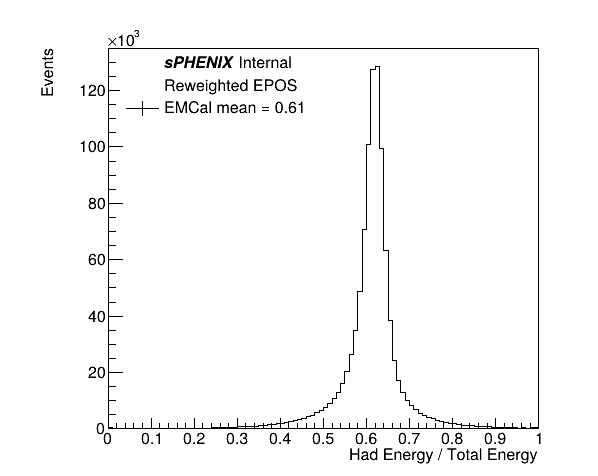
\includegraphics[width=0.48\linewidth]{detdeta/Figures/hadronic_fraction_syst/had_frac_emcal.png}
    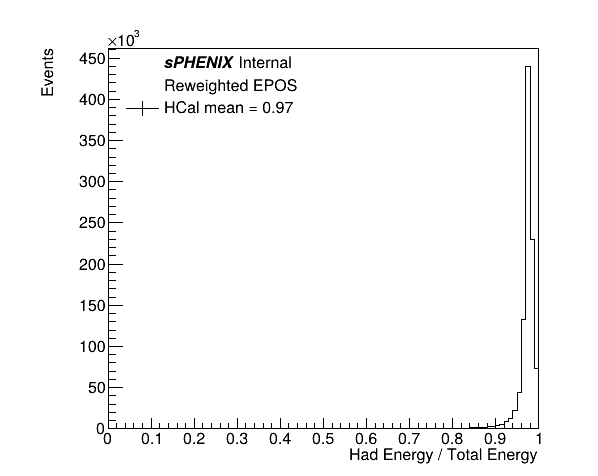
\includegraphics[width=0.48\linewidth]{detdeta/Figures/hadronic_fraction_syst/had_frac_hcal.png}
    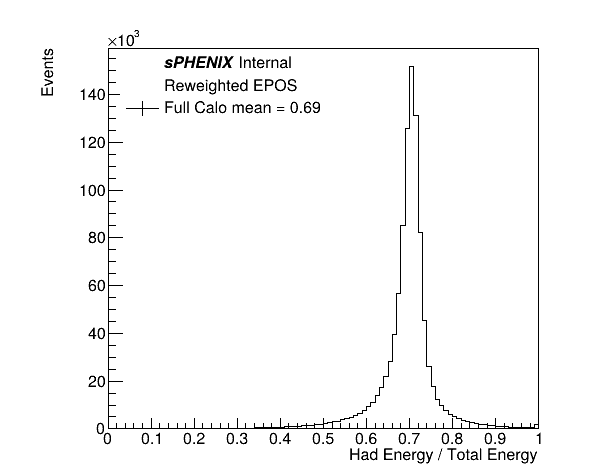
\includegraphics[width=0.48\linewidth]{detdeta/Figures/hadronic_fraction_syst/had_frac_calo.png}
    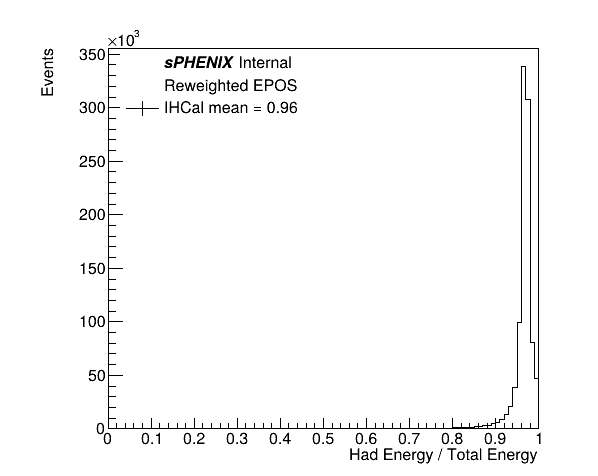
\includegraphics[width=0.48\linewidth]{detdeta/Figures/hadronic_fraction_syst/had_frac_ihcal.png}
    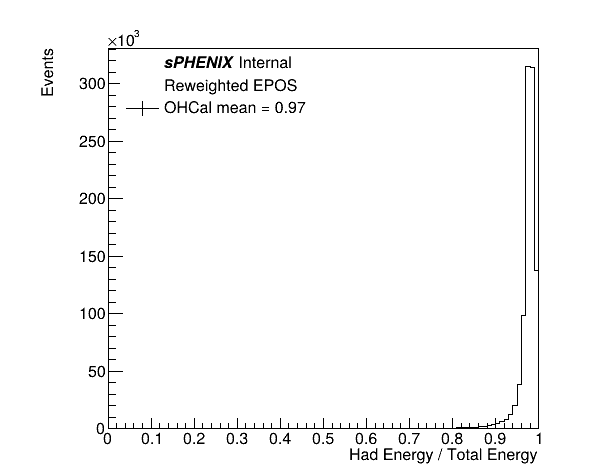
\includegraphics[width=0.48\linewidth]{detdeta/Figures/hadronic_fraction_syst/had_frac_ohcal.png}
    \caption{Ratio of hadronic energy in each particular layer of the calorimeter to the total energy (EM + hadronic) in that calorimeter layer found from reweighted \epos events shown for EMCal (top left), HCal (top right), full calorimeter (middle left), IHCal-only (middle right) and OHCal-only (bottom).}
    \label{fig:hadronic_fraction_syst}
\end{figure}

Additional simulation-based cross checks of the hadronic response uncertainty were undertaken using the full sPHENIX \geant simulation and the results of these studies have been used to verify that the hadronic uncertainty determined from test beam studies of the standalone HCal are suitable to be applied to the EMCal and full calorimeter \detdeta measurements.
These studies showed that the response variation due to variations in \geant modeling of hadronic showers is very comparable between the EMCal, full calorimeter and HCal. 

Three datasets of minimum bias \epos events were simulated in the sPHENIX \geant simulation using variations of the \geant physics lists discussed previously: "FTFP\_BERT", "FTFP\_BERT\_HP" and "QGSP\_BERT\_HP"~\cite{FTFP_BERT_model,QGSP_BERT_model}.
The reconstructed \detdeta value for each calorimeter was compared across the simulation datasets with different physics configuration lists and the largest difference between \detdeta values over the measurement $\eta$ range to determine the effect of using different physics configurations on the measurement. 
This corresponds to a variation of 3\% in the EMCal \detdeta results, 2-3\% in the IHCal \detdeta results and 3-4\% in the OHCal \detdeta results (Figure \ref{fig:phys_list_comp}).
The similarity in EMCal, HCal and full calorimeter response to changes in the physics configuration list in \geant provides confidence that the conservative test beam hadronic response uncertainty is applicable to the EMCal, HCal and full calorimeter measurements. 

\begin{figure}
    \centering
    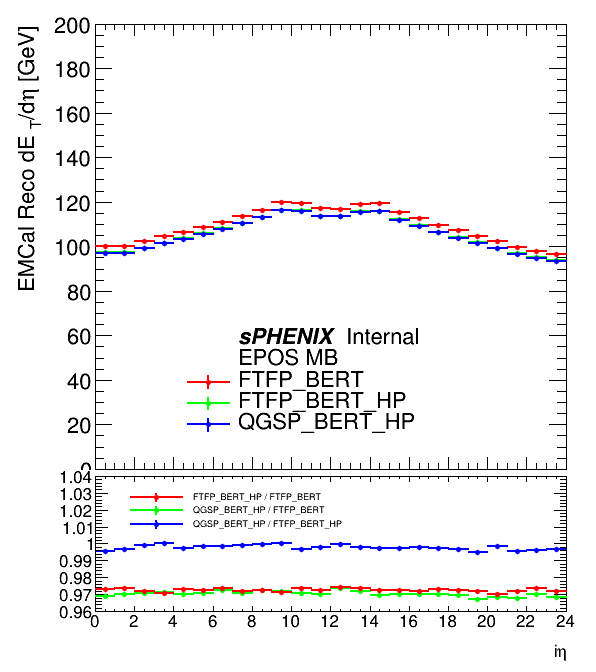
\includegraphics[width=0.48\linewidth]{detdeta/Figures/physics_lists_comp/emcal_reco_w_ratio_epos_mb_phys_list_comp.png}
    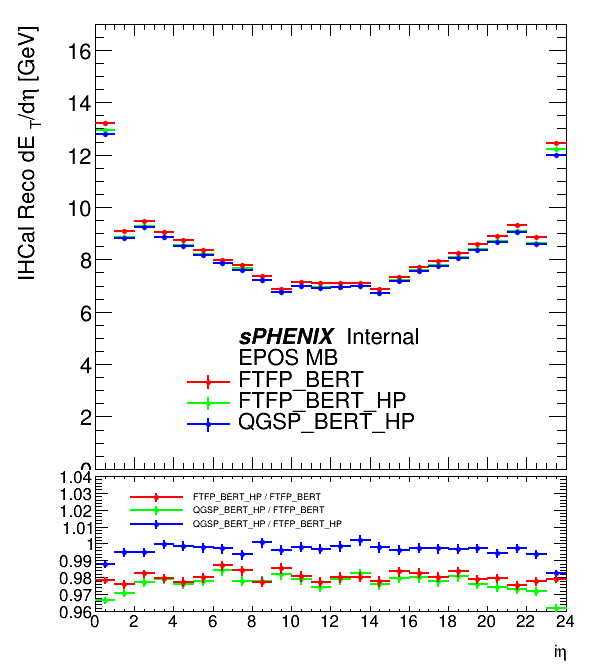
\includegraphics[width=0.48\linewidth]{detdeta/Figures/physics_lists_comp/ihcal_reco_w_ratio_epos_mb_phys_list_comp.png}
    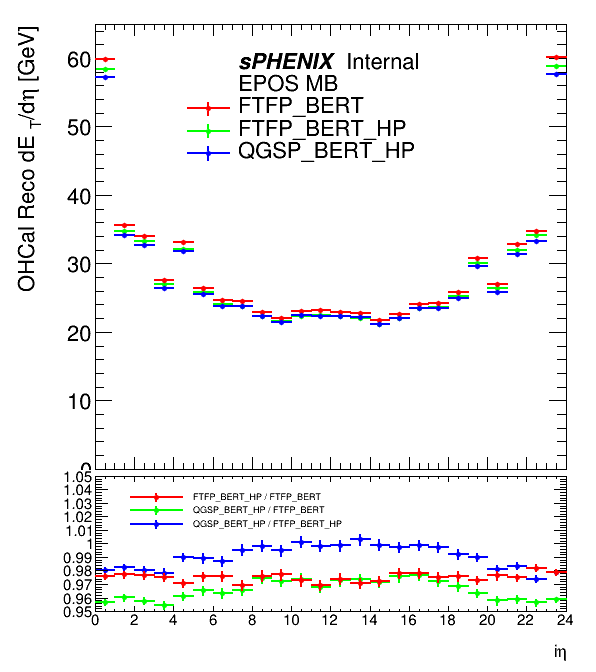
\includegraphics[width=0.48\linewidth]{detdeta/Figures/physics_lists_comp/ohcal_reco_w_ratio_epos_mb_phys_list_comp.png}
    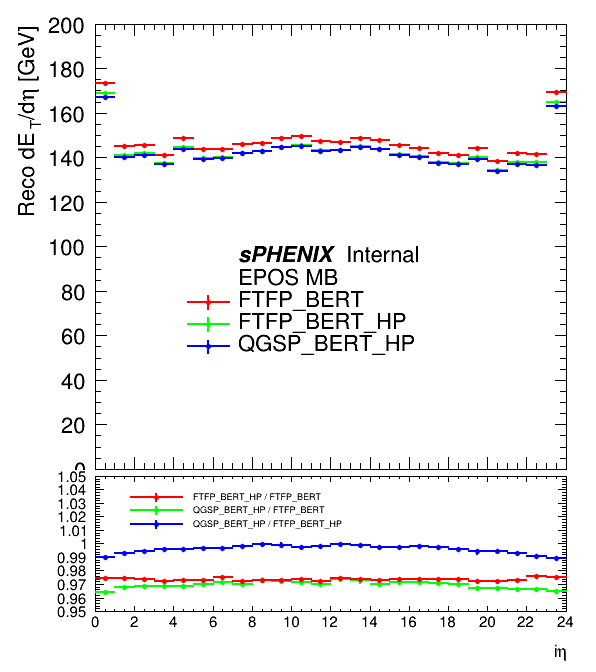
\includegraphics[width=0.48\linewidth]{detdeta/Figures/physics_lists_comp/calo_reco_w_ratio_epos_mb_phys_list_comp.png}
    \caption{Reconstructed \detdeta measurements as a function of HCal-tower $\eta$ binning for EMCal (top left), IHCal (top right), OHCal (bottom left) and full calorimeter (bottom right) in simulation. The HCal-tower $i\eta$ bin size is $\Delta\eta \approx 0.1$ and a total of 24 $i\eta$ bins comprise the measurement range. Comparison between different physics configuration lists, FTFP\_BERT, FTFP\_BERT\_HP and QGSP\_BERT\_HP.}
    \label{fig:phys_list_comp}
\end{figure}

\subsection{MC Reweighting}
To estimate the uncertainty associated with the MC reweighting scheme applied to the simulation datasets used for deriving the \detdeta correction factors, the reweighting scheme is applied to all three MC generators, \epos, \ampt and \hijing.
The data is first corrected using the nominal correction factors from the reweighted \epos sample, then the data is corrected using the variation correction factors from the reweighted \hijing and \ampt samples.
The average variation from the nominal measurement is extracted as a systematic on the MC particle composition reweighting methodology for each of the fully corrected \detdeta measurements at each $\eta$ value over the full $\eta$ measurement region. 
Considering the very different final state particle compositions as a function of centrality for these three generators as seen in Section~\ref{sec:detdeta_mcsamples}, any under- or over-estimates of the average energy contributions from identified particles in the \detdeta measurement after the reweighting methodology should be included in the difference in correction factors from these variations. 

Since the nominal correction factors use a particle spectra reweighting scheme that is only dependent on $p_{\text{T}}$ and centrality, an additional method of particle spectra reweighting which is differential in both transverse momentum and rapidity is implemented as a variation.
This rapidity dependent reweighting tests how robust the \detdeta correction factors are to particle spectra differences as a function of rapidity within the measurement pseudorapidity range $|\eta| <$ 1.1. 

For this rapidity dependent MC particle reweighting, the data/MC ratio of particle yield in central collisions (0-5\%) as a function of rapidity used data from the BRAHMS~\cite{Brahms_pi_spectra,Brahms_p_spectra} experiment. 
This data/MC ratio as a function of rapidity is applied as a rapidity dependent adjustment to the nominal $p_{\text{T}}$ and centrality dependent corrections, originally derived using mid-rapidity data.

From simulation studies it was determined that forward $\eta$ calorimeter towers ($0.8 < |\eta| < 1.1$) in sPHENIX see a large fraction of forward $\eta$ particles either directly from the collision or as secondary particles from showers in the support structures at very forward $\eta$. 
Therefore, incorporating this rapidity-dependent variation is valuable especially for the \detdeta measurement at forward $\eta$. 
The rapidity dependence uncertainty on the MC reweighting has an effect of at most 5.5\% in the most forward towers of the HCal, which agrees with the simulation studies on the location of the largest contributions from forward $\eta$ particles.
In the EMCal, this MC rapidity dependent reweighting variation has at most a 2.8\% effect, also in the most forward towers of the EMCal.
The MC rapidity dependent reweighting variation has at most a 4\% effect in the full calorimeter measurement. 
A plot of the \detdeta uncertainty as a function of $\eta$ from varying the MC reweighting rapidity dependence is included in Figure \ref{fig:mc_rap_dep}.

\begin{figure}
    \centering
    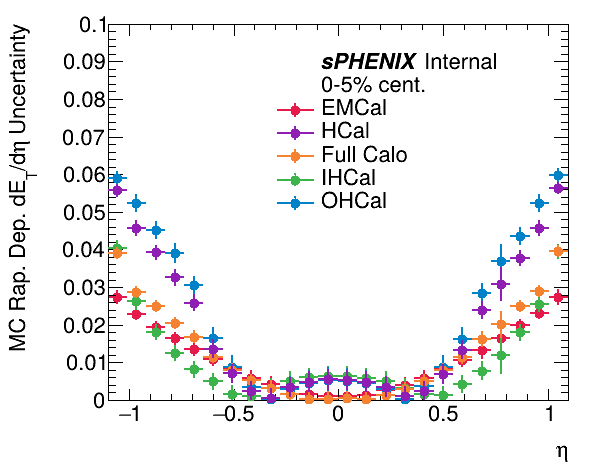
\includegraphics[width=0.5\linewidth]{detdeta/Figures/mc_generator_syst/MC_rap_dep_syst.png}
    \caption{Relative uncertainty in MC particle spectra reweighting rapidity dependence found from relative variation on the \detdeta measurement when using rapidity dependent correction to MC-weighting scheme. Nominal MC correction factor is weighted using weighting factors derived from mid-rapidity particle spectra from PHENIX and STAR. Variation MC correction factor has additional weighting factor differential in rapidity which comes from data/MC ratios derived from rapidity dependent spectra from BRAHMS~\cite{Brahms_pi_spectra,Brahms_p_spectra}.}
    \label{fig:mc_rap_dep}
\end{figure}

Therefore, the systematic uncertainty on the MC-derived correction factors is comprised of these two contributions: the uncertainty on the reweighting methodology determined by reweighting multiple generators and the uncertainty on the rapidity dependence of the reweighting scheme found by toggling rapidity dependent and independent reweighting factors.
The overall effect of the MC reweighting uncertainty on the \detdeta measurement integrated over $\eta$ for different centrality bins is 1.4-2.1\% for the EMCal \detdeta measurement, 2.5-3.8\% for the HCal \detdeta measurement, and 1.6-2.2\% for the full calorimeter \detdeta measurement. 
The HCal \detdeta measurement is the most sensitive to both the reweighting methodology and the $\eta$ dependence of the particle spectra used for the MC reweighting factors.

\subsection{Zero Suppression Application}
As described in Section \ref{sec:nominal_calorimeter_reconstruction}, within the calorimeter reconstruction pipeline, a zero suppression algorithm is used for processing both the low energy signals and noise. 
To test the robustness of the \detdeta measurements to noise processing using the zero suppression algorithm versus the template fit method, the ADC threshold at which the switch from waveform processing using zero suppression to using the template fit is varied. 
The ADC threshold is varied from the nominal thresholds of 100(50) ADC for the EMCal(HCal) to thresholds of 200(100) ADC and 60(30) ADC for the EMCal(HCal). 
For \detdeta results from the EMCal, varying the ZS application threshold has a 1.0-5.8\% effect, with the effect growing in more peripheral events. 
There is a 0.2\% effect on the HCal \detdeta results and 0.8-4.4\% effect on the full calorimeter \detdeta results. 

It is expected that the EMCal measurement would be most sensitive to changes in the ZS threshold since the EMCal has a much higher overall level of noise compared to the HCal and the ZS threshold determines how much noise is processed using the template fit method in the calorimeter tower reconstruction.
Biases from processing noise with the template fit method were studied in depth using Run 2023 data and are included in Section~\ref{sec:zerosuppression}.
Therefore, it is expected that varying the zero suppression to template fit switching threshold would have the largest impact on the EMCal as well as a larger impact in peripheral events where the ratio of signal to noise in the calorimeters should be smaller than in central events. 
The EMCal also has an asymmetric noise distribution as a function of $\eta$ with higher noise levels at positive $\eta$ compared to negative $\eta$ due to the yellow beam having higher backgrounds than the blue beam in the sPHENIX detector.
This asymmetric noise distribution in the EMCal causes the asymmetric ZS threshold variation effect as a function of $\eta$ seen in the peripheral centrality bins of Figures~\ref{fig:eta_dep_syst_emcal} and \ref{fig:eta_dep_syst_calo} when the ZS threshold variation becomes a dominant systematic uncertainty. 

\subsection{Detector Acceptance} 
To determine the effect of the changing calorimeter acceptance run by run on the \detdeta measurement, the fully corrected \detdeta for the nominal dataset is compared to two variation runs. 
The run by run variation is determined for each centrality bin and uses run-specific correction factors from the reweighted \epos MC sample determined from run-specific bad tower masks (shown in Figure~\ref{fig:bad_tower_masks_detdeta}) as well as run-specific MC vertex reweighting factors. 
Both the nominal dataset and the variation runs are taken within the same beam fill and have the same calorimeter absolute EM-scale calibration factors applied. 
Therefore, the remaining variation for these run by run differences should be due to the run by run differences in acceptance. 
Figure~\ref{fig:calo_run_variation} shows the run by run \detdeta measurements for 0-5\% central events of runs in this run group and the effect of changing calorimeter acceptance.
This effect is very small, on the level of less than 0.5\%, for all calorimeter \detdeta measurements.
 
\begin{figure}
    \centering
    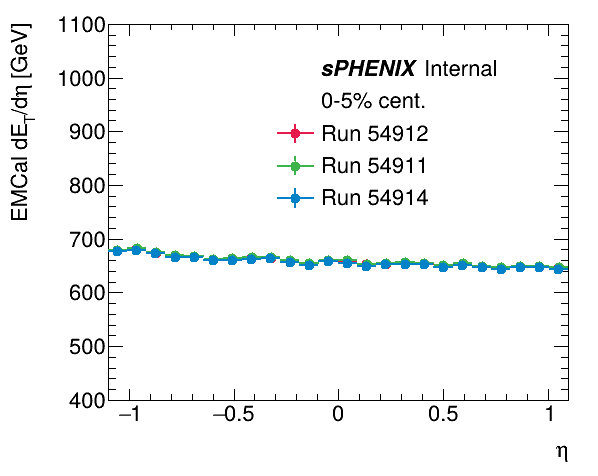
\includegraphics[width=0.48\linewidth]{detdeta/Figures/detector_acceptance_syst/run_by_run_emcal_0-5.png}
    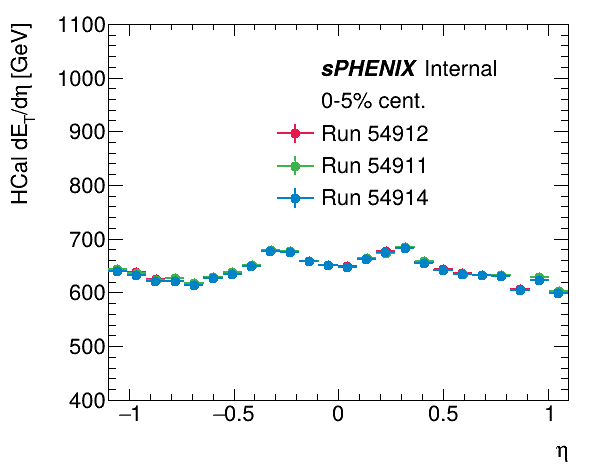
\includegraphics[width=0.48\linewidth]{detdeta/Figures/detector_acceptance_syst/run_by_run_hcal_0-5.png}
    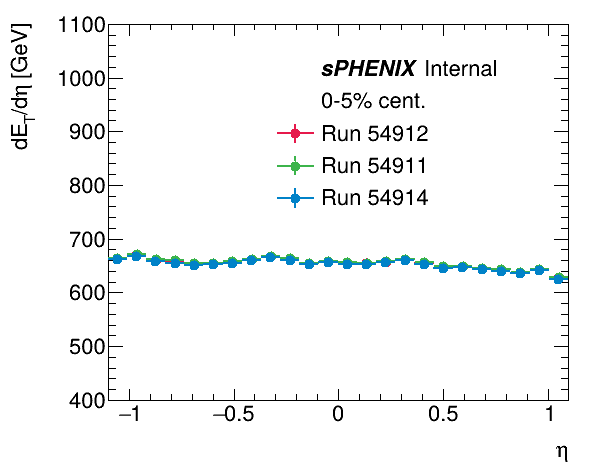
\includegraphics[width=0.48\linewidth]{detdeta/Figures/detector_acceptance_syst/run_by_run_calo_0-5.png}
    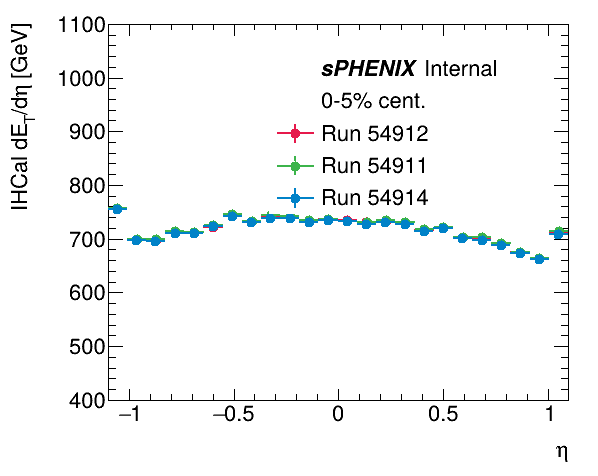
\includegraphics[width=0.48\linewidth]{detdeta/Figures/detector_acceptance_syst/run_by_run_ihcal_0-5.png}
    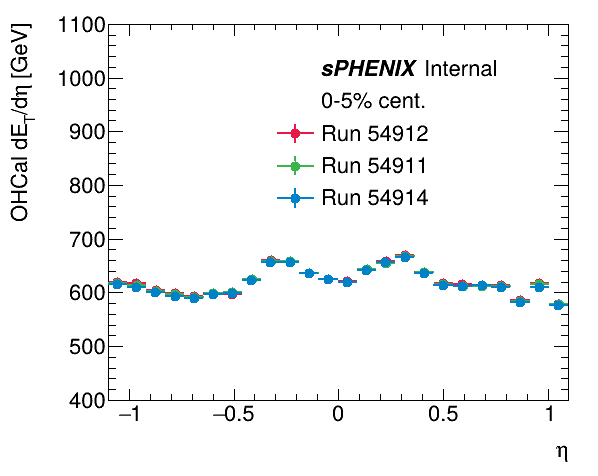
\includegraphics[width=0.48\linewidth]{detdeta/Figures/detector_acceptance_syst/run_by_run_ohcal_0-5.png}
    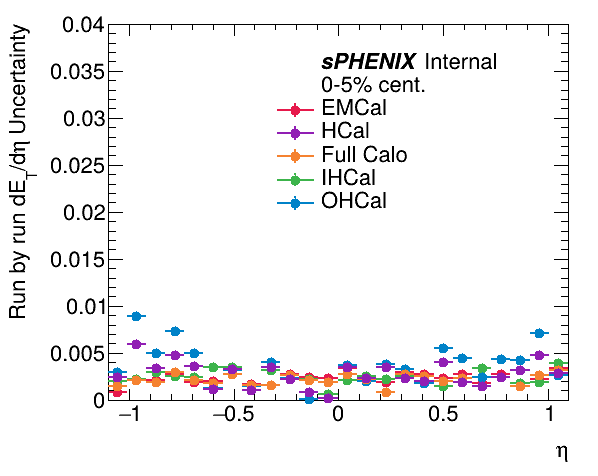
\includegraphics[width=0.48\linewidth]{detdeta/Figures/detector_acceptance_syst/run_by_run_syst_0-5.png}
    \caption{Fully corrected \detdeta results shown for 0-5\% centrality bin using data from EMCal (top left), HCal (top right), full calorimeter (middle left), IHCal-only (middle right) and OHCal (bottom left) from 3 different runs of the measurement dataset. The average relative variation as a function of $\eta$ for each calorimeter measurement shown in \detdeta uncertainty plot (bottom right).}
    \label{fig:calo_run_variation}
\end{figure}

\subsection{Z-vertex Uncertainty}
For all events used in this study, the z-vertex was determined using the MBD, which was determined to have a z-vertex resolution of less than 1 cm in central Au+Au events and about 2.5 cm in peripheral Au+Au events \cite{Lis1}. 
To study the effect of this MBD z-vertex resolution on the \detdeta measurement, the z-vertex is shifted by a conservative 3 cm for all events and the full analysis chain is reproduced.
For all calorimeter measurements, this z-vertex shift has $< 0.5\%$ effect on the \detdeta measurement. 

\subsection{\Npart Uncertainty}
For measurements of \detdeta as a function of \Npart, an additional uncertainty on the mean \Npart value for a centrality range is included. 
Uncertainties on the extracted $\left<\Npart\right>$ values were evaluated using a standard set of variations in the MC Glauber modeling and centrality determination~\cite{Lis1}. 
These include varying the nucleon--nucleon cross-section and other geometric parameters in the Glauber model and varying centile cuts according to the uncertainty in the total efficiency. 
However, the dominant source of uncertainty for the  $\left<\Npart\right>$ values was the uncertainty in the MB trigger efficiency, which includes the previously discussed contributions from simulation studies of the MBD trigger efficiency and studies with and without the coincidence hits in the ZDC included the minbias definition. 
For the centrality intervals used in this measurement, the uncertainties ranged from $0.6$\% in $0$--$5$\% events to $13.8$\% in $60$--$70$\% events. 

\subsection{Total Systematic Uncertainty}

The total systematic uncertainties for \detdeta are found as a function of $\eta$ for the EMCal, HCal and full calorimeter measurement for each centrality bin and are shown in Figures ~\ref{fig:eta_dep_syst_emcal}, \ref{fig:eta_dep_syst_hcal} and \ref{fig:eta_dep_syst_calo}. 
The total systematic uncertainty as well as contributing uncertainties averaged over the full $-1.1 < \eta < 1.1$ measurement range are shown in Table \ref{table:SystUncertainties} for all centrality bins.
Additional systematic uncertainty results for the IHCal-only and OHCal-only \detdeta measurements as a function of $\eta$ are included in Appendix~\ref{sec:detdeta_add_syst}.
The averaged total uncertainty on \detdeta from EMCal data is between 5.3\% and 8.1\%. The uncertainty on the EMCal \detdeta measurement increases when moving to more peripheral centrality bins. 
For all centrality bins, largest uncertainty contribution on the EMCal \detdeta measurement comes from the uncertainty in the calorimeter's hadronic response. 
However, in more peripheral centrality bins, the uncertainty due to noise processing is also a major source of uncertainty on the EMCal \detdeta measurement. 
The total uncertainty on \detdeta from HCal data is consistently between 7.7\% and 8.3\% across all centrality bins. 
The largest source of uncertainty on the HCal \detdeta measurement also comes from the uncertainty on the hadronic response while the second largest uncertainty comes from the uncertainty on the MC correction factors. 
The total uncertainty on the full calorimeter measurement of \detdeta ranges between 5.6\% and 7.4\% and, similar to the EMCal measurement, the full calorimeter uncertainties increase when moving to more peripheral bins. 
The full calorimeter uncertainty is dominated by the hadronic response uncertainty for all centrality bins with uncertainty on the noise becoming a second major source of uncertainty in more peripheral centrality bins.

\begin{table}
\centering
\begin{tabular}{ |p{1.3cm}|p{2.1cm}|p{1.0cm}|p{1.0cm}|p{1.0cm}|p{1.0cm}|p{1.3cm}|p{1.0cm}|p{1.0cm}|  }
\hline
& & \raggedright Calib. & \raggedright Had. resp. & \raggedright MC & ZS & Accept. & Glob. & Total \\
\hline
\multirow{4}{*}{0-5\%} & EMCal   & 2.6  & 4.1 & 1.4 & 1.0 & 0.2 & 0.3 & 5.3 \\
& HCal                           & 2.7  & 6.6 & 2.9 & 0.3 & 0.3 & 0.1 & 7.9 \\
& Full Calo                      & 2.1  & 4.7 & 1.8 & 0.8 & 0.2 & 0.2 & 5.6 \\
& IHCal-only                     & 10.0 & 6.5 & 1.6 & 0.1 & 0.2 & 0.4 & 12.1 \\
& OHCal-only                     & 1.0  & 6.6 & 3.3 & 0.4 & 0.4 & 0.1 & 7.7 \\
\hline
\multirow{4}{*}{5-10\%}& EMCal   & 2.6  & 4.1 & 1.4 & 1.2 & 0.2 & 0.3 & 5.3 \\
& HCal                           & 2.7  & 6.6 & 2.7 & 0.2 & 0.3 & 0.1 & 7.8 \\
& Full Calo                      & 2.1  & 4.7 & 1.7 & 0.9 & 0.2 & 0.2 & 5.6 \\
& IHCal-only                     & 10.0 & 6.5 & 1.5 & 0.1 & 0.3 & 0.4 & 12.1 \\
& OHCal-only                     & 1.0  & 6.6 & 3.1 & 0.3 & 0.3 & 0.1 & 7.7 \\
\hline
\multirow{4}{*}{10-20\%}& EMCal  & 2.6  & 4.1 & 1.4 & 1.3 & 0.4 & 0.3 & 5.3 \\
& HCal                           & 2.7  & 6.6 & 2.5 & 0.2 & 0.3 & 0.1 & 7.7 \\
& Full Calo                      & 2.1  & 4.7 & 1.6 & 1.0 & 0.3 & 0.2 & 5.6 \\
& IHCal-only                     & 10.0 & 6.5 & 1.4 & 0.1 & 0.4 & 0.4 & 12.1 \\
& OHCal-only                     & 1.0  & 6.6 & 2.9 & 0.3 & 0.3 & 0.1 & 7.5 \\
\hline
\multirow{4}{*}{20-30\%}& EMCal  & 2.6  & 4.1 & 1.4 & 1.6 & 0.3 & 0.3 & 5.4 \\
& HCal                           & 2.7  & 6.6 & 2.5 & 0.2 & 0.2 & 0.1 & 7.7 \\
& Full Calo                      & 2.1  & 4.7 & 1.6 & 1.2 & 0.2 & 0.2 & 5.7 \\
& IHCal-only                     & 10.0 & 6.5 & 1.3 & 0.1 & 0.3 & 0.4 & 12.1 \\
& OHCal-only                     & 1.0  & 6.6 & 2.8 & 0.3 & 0.3 & 0.1 & 7.7 \\
\hline
\multirow{4}{*}{30-40\%}& EMCal  & 2.6  & 4.1 & 1.4 & 2.0 & 0.2 & 0.3 & 5.5 \\
& HCal                           & 2.7  & 6.6 & 2.5 & 0.2 & 0.4 & 0.1 & 7.7 \\
& Full Calo                      & 2.1  & 4.7 & 1.6 & 1.5 & 0.1 & 0.2 & 5.7 \\
& IHCal-only                     & 10.0 & 6.5 & 1.4 & 0.1 & 0.2 & 0.4 & 12.1 \\
& OHCal-only                     & 1.0  & 6.6 & 2.9 & 0.2 & 0.5 & 0.2 & 7.5 \\
\hline
\multirow{4}{*}{40-50\%}& EMCal  & 2.6  & 4.1 & 1.6 & 2.5 & 0.2 & 0.3 & 5.9 \\
& HCal                           & 2.7  & 6.6 & 2.8 & 0.2 & 0.4 & 0.2 & 7.8 \\
& Full Calo                      & 2.1  & 4.7 & 1.8 & 1.9 & 0.2 & 0.3 & 5.9 \\
& IHCal-only                     & 10.0 & 6.5 & 1.8 & 0.1 & 0.3 & 0.5 & 12.1 \\
& OHCal-only                     & 1.0  & 6.6 & 3.1 & 0.2 & 0.5 & 0.2 & 7.6 \\
\hline
\multirow{4}{*}{50-60\%}& EMCal  & 2.6  & 4.1 & 1.8 & 3.6 & 0.4 & 0.4 & 6.5 \\
& HCal                           & 2.7  & 6.6 & 3.0 & 0.2 & 0.4 & 0.2 & 7.9 \\
& Full Calo                      & 2.1  & 4.7 & 1.9 & 2.7 & 0.3 & 0.3 & 6.3 \\
& IHCal-only                     & 10.0 & 6.5 & 2.1 & 0.1 & 0.4 & 0.5 & 12.2 \\
& OHCal-only                     & 1.0  & 6.6 & 3.4 & 0.3 & 0.5 & 0.2 & 7.8 \\
\hline
\multirow{4}{*}{60-70\%}& EMCal  & 2.6  & 4.1 & 2.1 & 5.8 & 0.5 & 0.4 & 8.1 \\
& HCal                           & 2.7  & 6.6 & 3.8 & 0.2 & 0.6 & 0.2 & 8.3 \\
& Full Calo                      & 2.1  & 4.7 & 2.2 & 4.4 & 0.3 & 0.3 & 7.4 \\
& IHCal-only                     & 10.0 & 6.5 & 2.6 & 0.1 & 0.6 & 0.5 & 12.3 \\
& OHCal-only                     & 1.0  & 6.6 & 4.3 & 0.3 & 0.7 & 0.3 & 8.2 \\
\hline
\end{tabular}
\caption{Summary of systematic uncertainties for \detdeta measurements averaged over the full $\eta$ measurement range ($-1.1 < \eta < 1.1$) for each calorimeter measurement for all centrality bins. Uncertainty values listed above are given in percentages.}
\label{table:SystUncertainties}
\end{table}

\begin{figure}
    \centering
    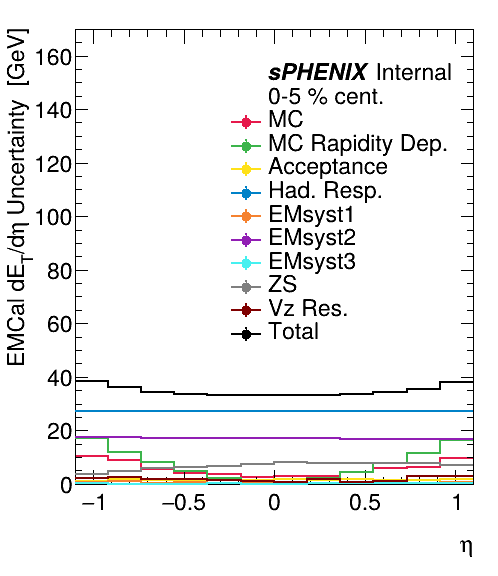
\includegraphics[width=0.32\linewidth]{figures/chapter4/emcal_total_syst_0-5.png}
    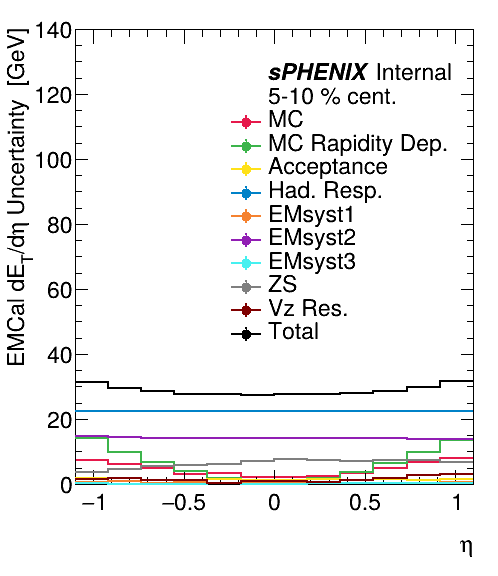
\includegraphics[width=0.32\linewidth]{figures/chapter4/emcal_total_syst_5-10.png}
    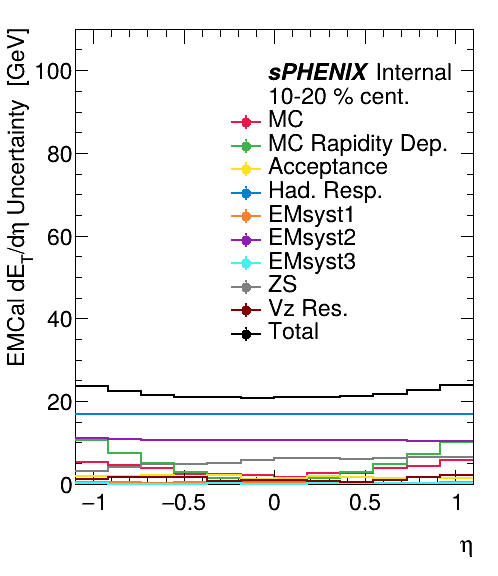
\includegraphics[width=0.32\linewidth]{figures/chapter4/emcal_total_syst_10-20.png}
    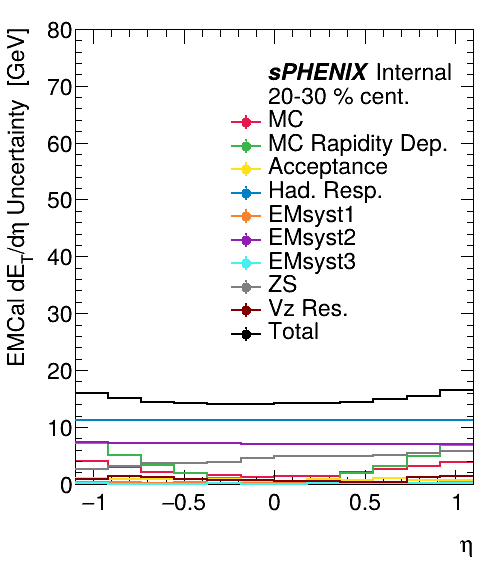
\includegraphics[width=0.32\linewidth]{figures/chapter4/emcal_total_syst_20-30.png}
    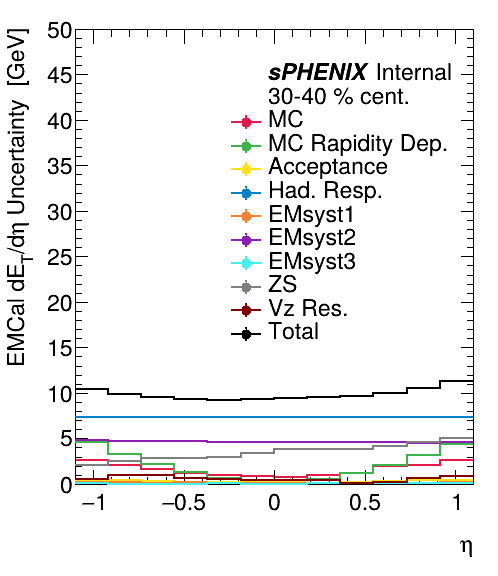
\includegraphics[width=0.32\linewidth]{figures/chapter4/emcal_total_syst_30-40.png}
    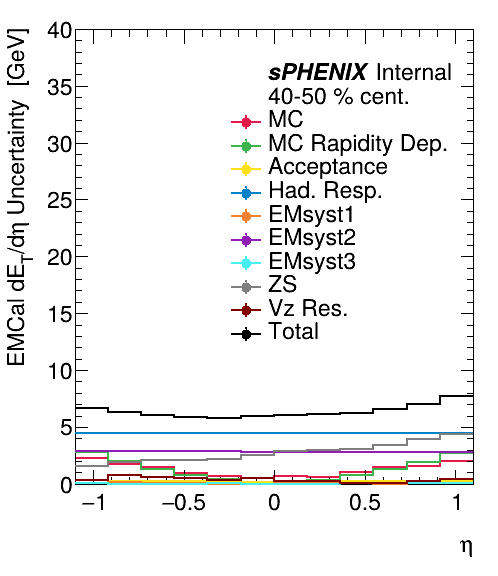
\includegraphics[width=0.32\linewidth]{figures/chapter4/emcal_total_syst_40-50.png}
    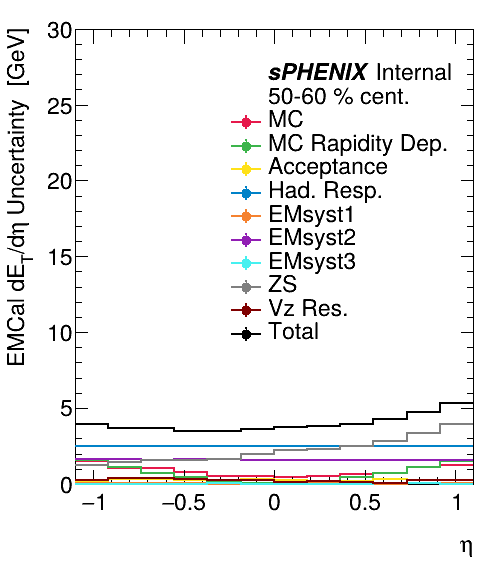
\includegraphics[width=0.32\linewidth]{figures/chapter4/emcal_total_syst_50-60.png}
    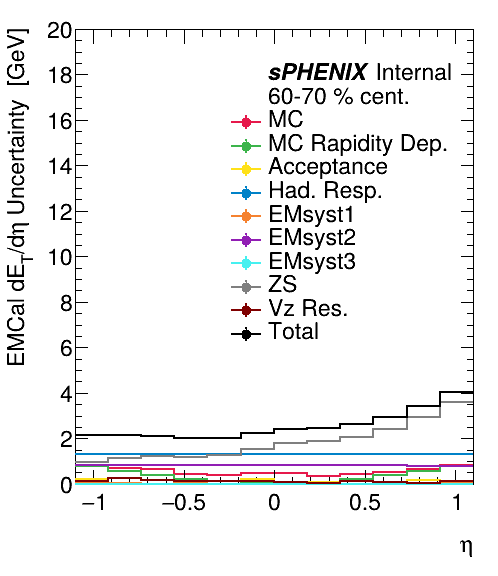
\includegraphics[width=0.32\linewidth]{figures/chapter4/emcal_total_syst_60-70.png}
    \caption{Absolute variation of systematic uncertainties on \detdeta measurements as a function of $\eta$ for \detdeta measurements from EMCal data. Uncertainties from all centralities in measurement are shown from central to peripheral events from top to bottom.}
    \label{fig:eta_dep_syst_emcal}
\end{figure}

\begin{figure}
    \centering
    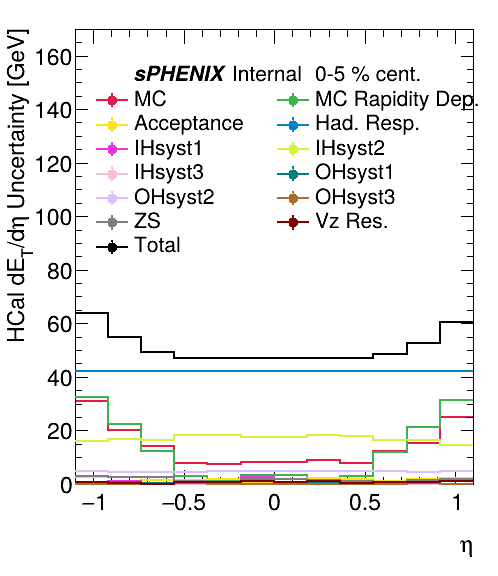
\includegraphics[width=0.32\linewidth]{figures/chapter4/hcal_total_syst_0-5.png}
    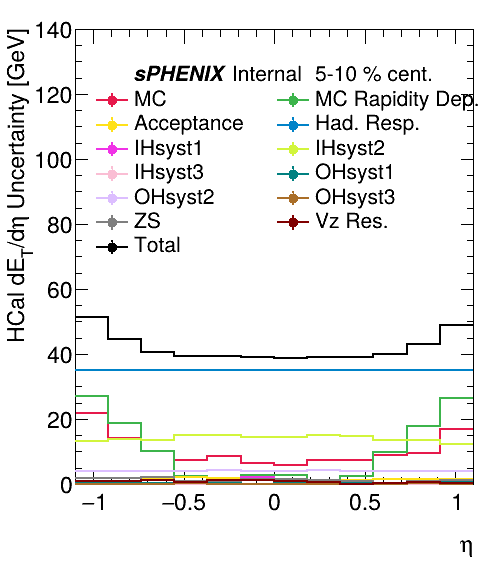
\includegraphics[width=0.32\linewidth]{figures/chapter4/hcal_total_syst_5-10.png}
    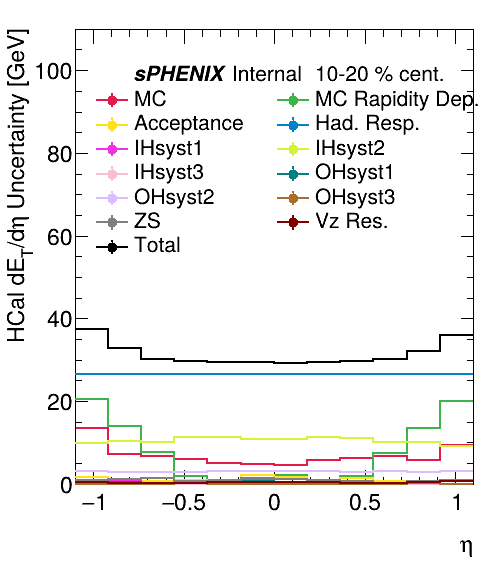
\includegraphics[width=0.32\linewidth]{figures/chapter4/hcal_total_syst_10-20.png}
    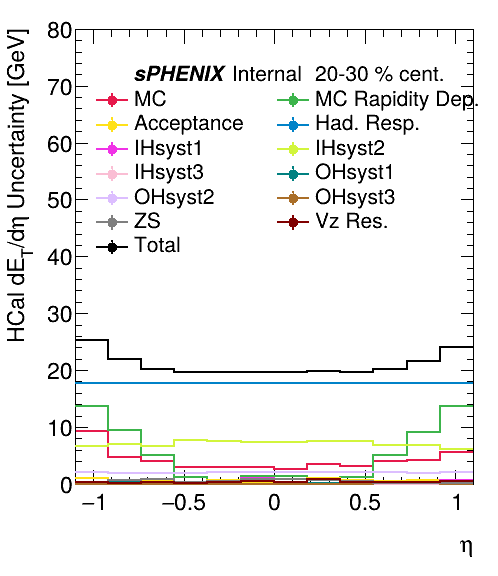
\includegraphics[width=0.32\linewidth]{figures/chapter4/hcal_total_syst_20-30.png}
    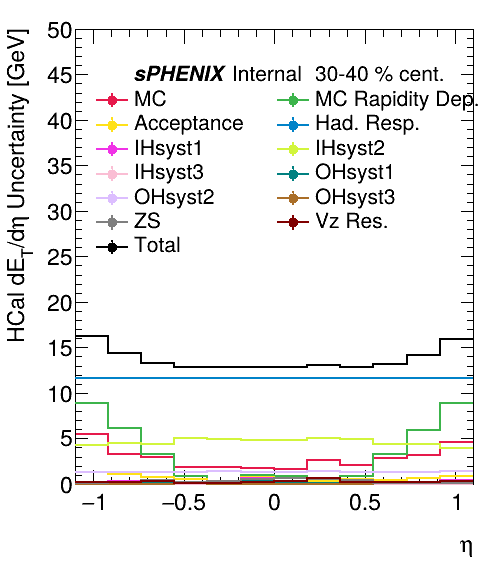
\includegraphics[width=0.32\linewidth]{figures/chapter4/hcal_total_syst_30-40.png}
    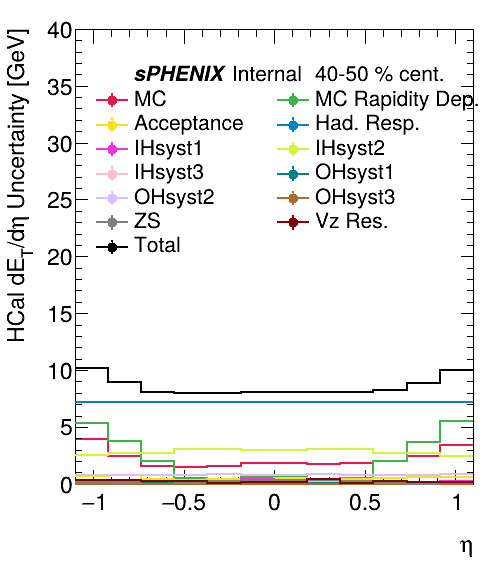
\includegraphics[width=0.32\linewidth]{figures/chapter4/hcal_total_syst_40-50.png}
    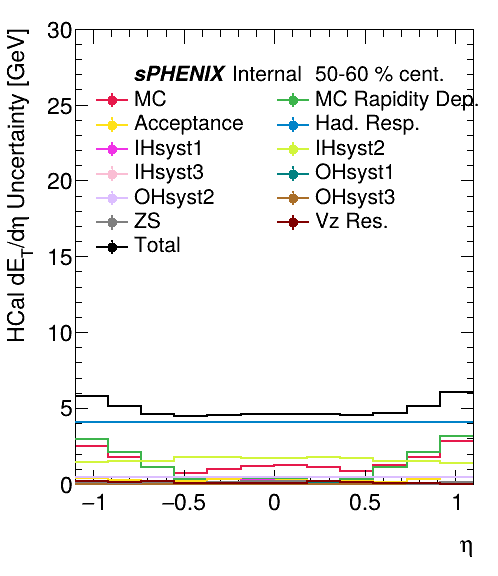
\includegraphics[width=0.32\linewidth]{figures/chapter4/hcal_total_syst_50-60.png}
    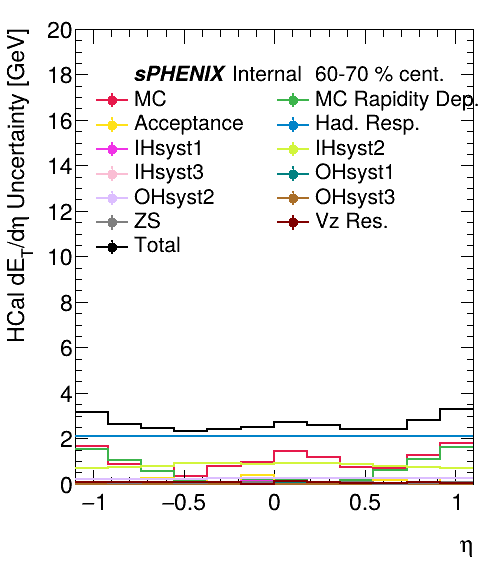
\includegraphics[width=0.32\linewidth]{figures/chapter4/hcal_total_syst_60-70.png}
    \caption{Absolute variation of systematic uncertainties on \detdeta measurements as a function of $\eta$ for \detdeta measurements from HCal data. Uncertainties from all centralities in measurement are shown from central to peripheral events from top to bottom.}
    \label{fig:eta_dep_syst_hcal}
\end{figure}

\begin{figure}
    \centering
    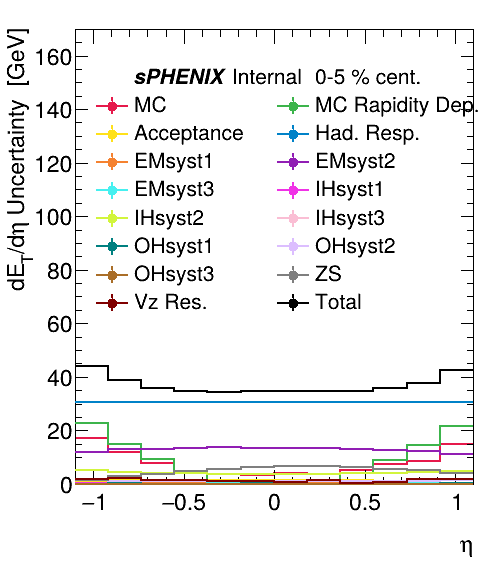
\includegraphics[width=0.32\linewidth]{figures/chapter4/calo_total_syst_0-5.png}
    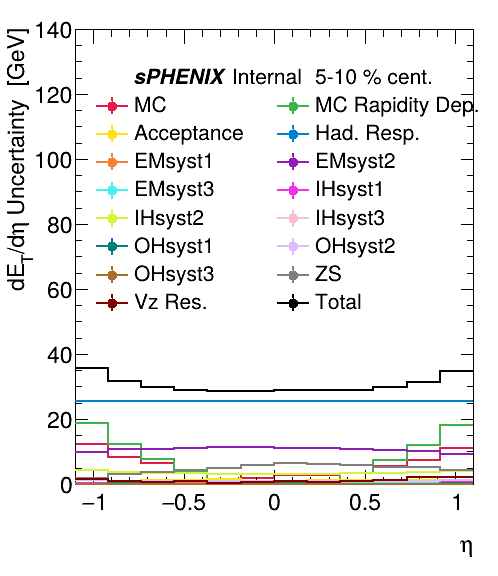
\includegraphics[width=0.32\linewidth]{figures/chapter4/calo_total_syst_5-10.png}
    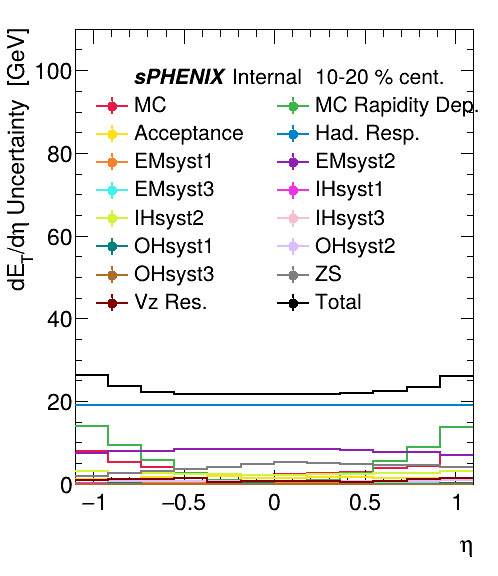
\includegraphics[width=0.32\linewidth]{figures/chapter4/calo_total_syst_10-20.png}
    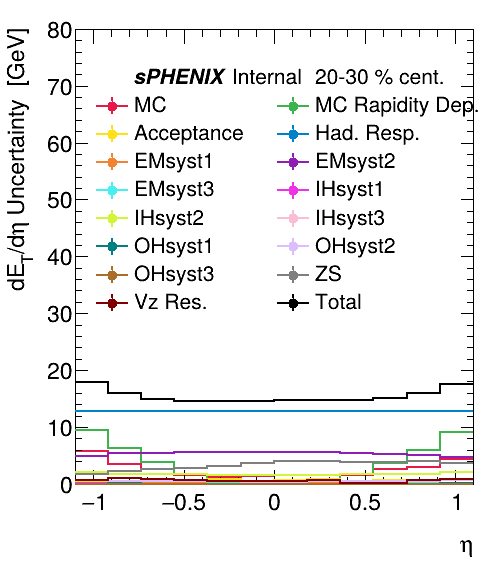
\includegraphics[width=0.32\linewidth]{figures/chapter4/calo_total_syst_20-30.png}
    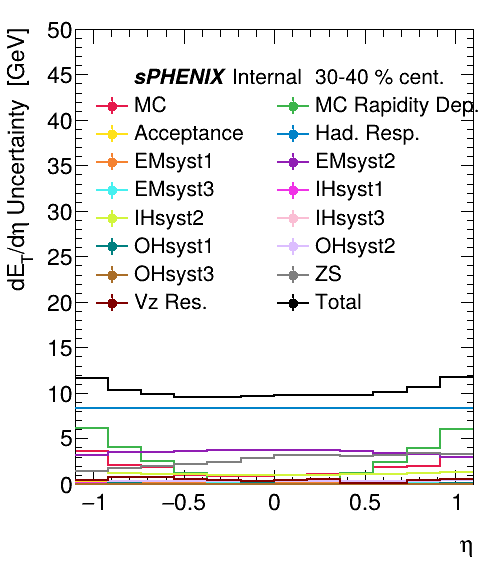
\includegraphics[width=0.32\linewidth]{figures/chapter4/calo_total_syst_30-40.png}
    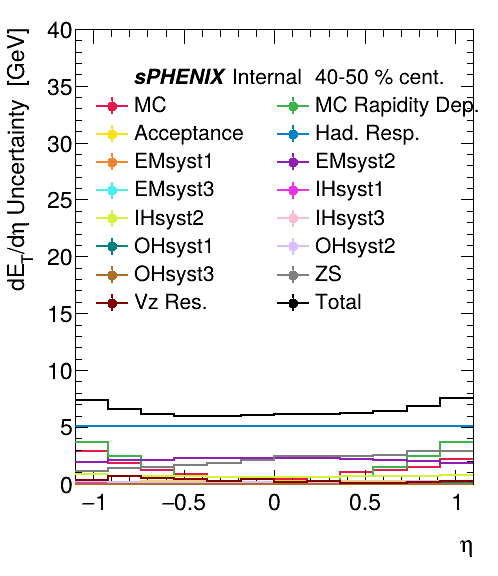
\includegraphics[width=0.32\linewidth]{figures/chapter4/calo_total_syst_40-50.png}
    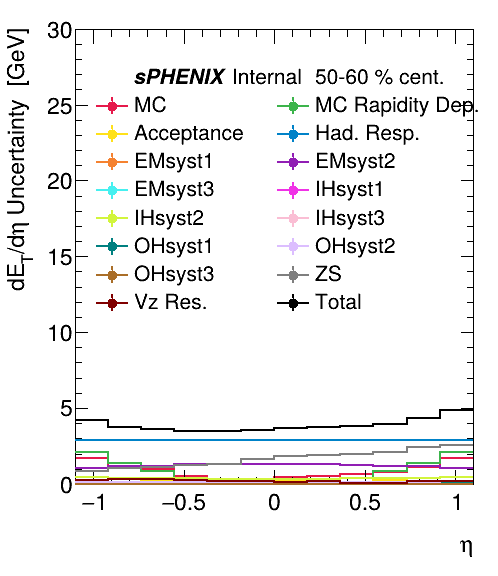
\includegraphics[width=0.32\linewidth]{figures/chapter4/calo_total_syst_50-60.png}
    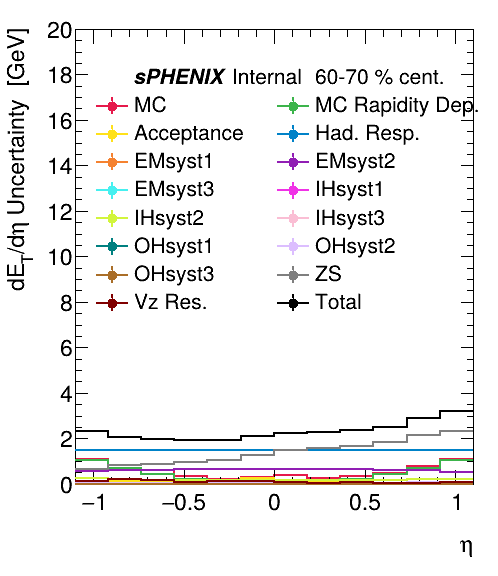
\includegraphics[width=0.32\linewidth]{figures/chapter4/calo_total_syst_60-70.png}
    \caption{Absolute variation of systematic uncertainties on \detdeta measurements as a function of $\eta$ for \detdeta measurements from full calorimeter data. Uncertainties from all centralities in measurement are shown from central to peripheral events from top to bottom.}
    \label{fig:eta_dep_syst_calo}
\end{figure}

\subsection{Correlated and Uncorrelated Systematic Uncertainties}

To make accurate statements on the consistency of \detdeta measurements made with different calorimeter systems and at different $\eta$ values, 
these measurements must be compared using only their uncorrelated uncertainties. 
However, many of the systematic uncertainties in the analysis are highly correlated in $\eta$, in centrality, as well as between different calorimeter layer measurements. 
The most dominant correlated uncertainty is the testbeam-based hadronic response uncertainty which is applied as a constant value across the full measurement range in $\eta$ and is applied as the same relative uncertainty for each centrality bin. 
Additionally, the hadronic response uncertainty for different calorimeter measurements (ie. EMCal-only, HCal-only and full calorimeter) is also highly correlated. 
The below description investigates the level of agreement within only uncorrelated systematic uncertainties between the EMCal-only and HCal-only measurements and between measurements of \detdeta at positive and negative $\eta$ for all calorimeter measurements.

\subsubsection{EMCal and HCal Agreement}

The level of correlation between the EMCal and HCal measurements is first determined by using all systematic variations in this analysis. 
Plots of the variation in EMCal \detdeta versus HCal \detdeta for each systematic variation and each centrality bin are shown in Figure~\ref{fig:emcal_hcal_covariance}. 
The Pearson correlation coefficient is extracted from these correlation plots; these correlation coefficients between the EMCal and HCal measurements for each centrality bin range from 0.77 to 0.59 as shown in Table~\ref{tab:emcal_hcal_correlation}.

\begin{figure}
    \centering
    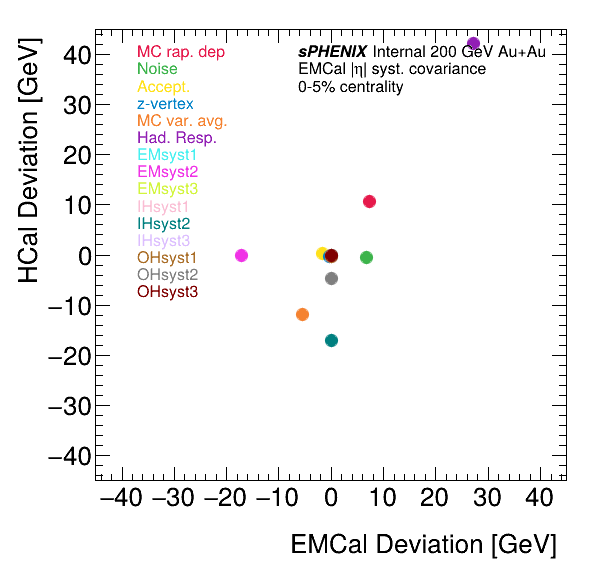
\includegraphics[width=0.32\linewidth]{detdeta/Figures/corr_syst_uncertainties/covariance_0-5.png}
    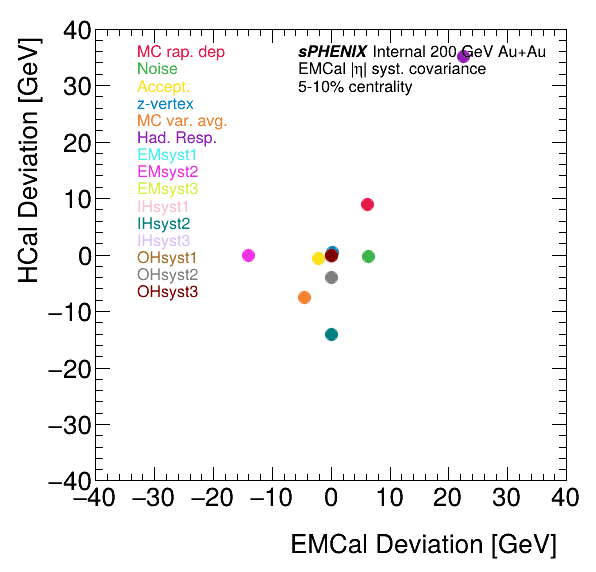
\includegraphics[width=0.32\linewidth]{detdeta/Figures/corr_syst_uncertainties/covariance_5-10.png}
    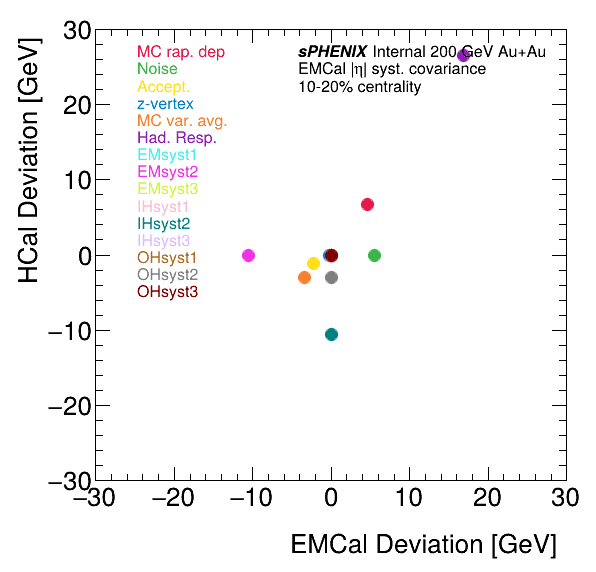
\includegraphics[width=0.32\linewidth]{detdeta/Figures/corr_syst_uncertainties/covariance_10-20.png}
    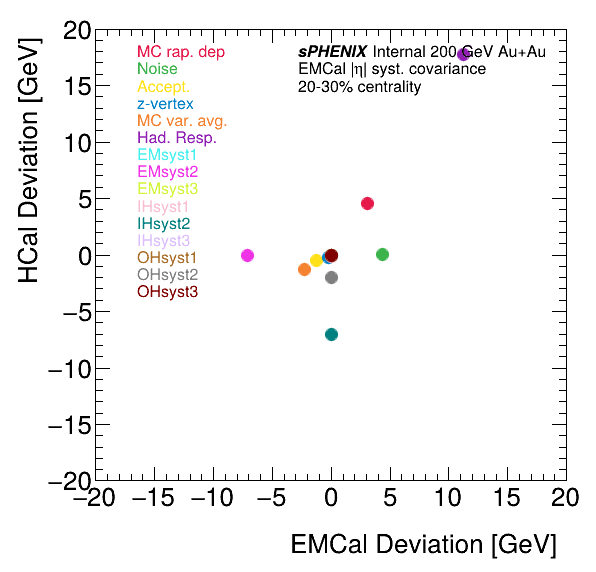
\includegraphics[width=0.32\linewidth]{detdeta/Figures/corr_syst_uncertainties/covariance_20-30.png}
    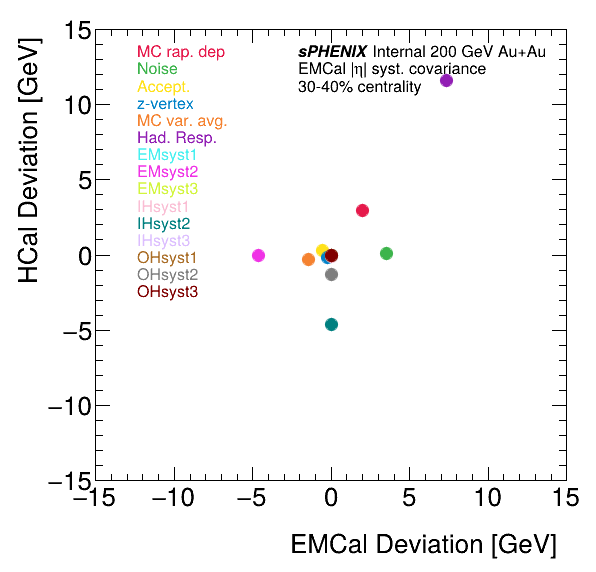
\includegraphics[width=0.32\linewidth]{detdeta/Figures/corr_syst_uncertainties/covariance_30-40.png}
    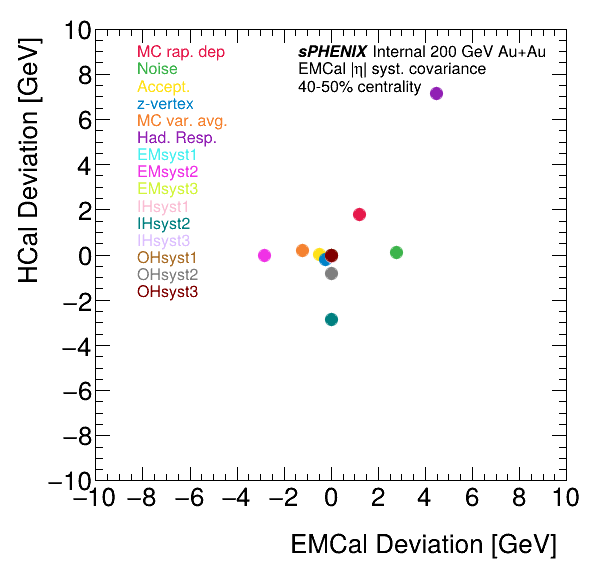
\includegraphics[width=0.32\linewidth]{detdeta/Figures/corr_syst_uncertainties/covariance_40-50.png}
    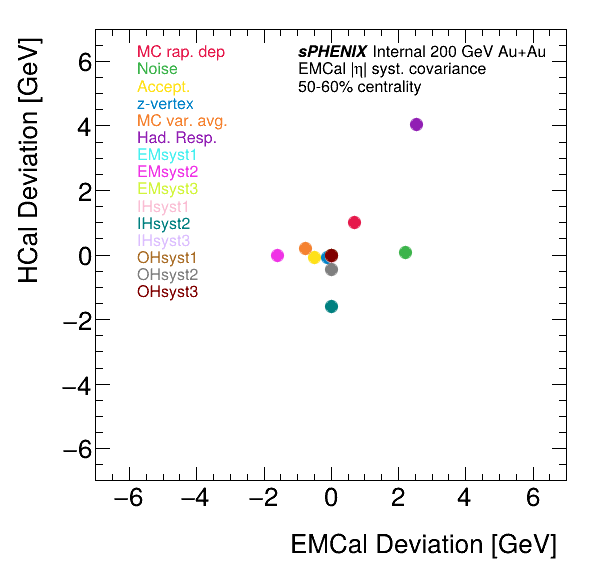
\includegraphics[width=0.32\linewidth]{detdeta/Figures/corr_syst_uncertainties/covariance_50-60.png}
    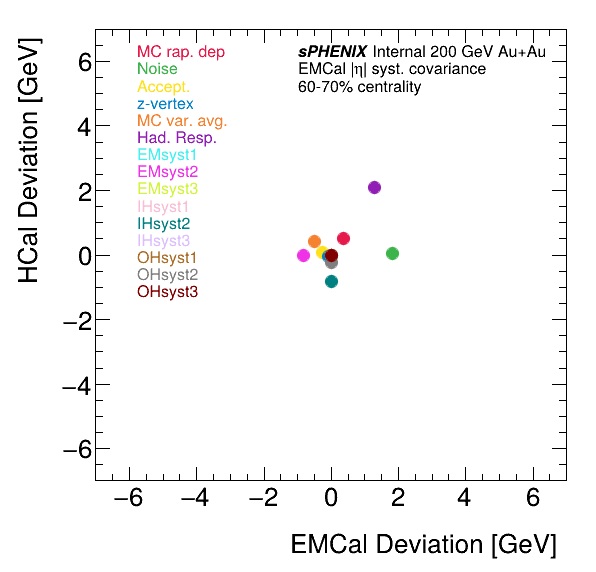
\includegraphics[width=0.32\linewidth]{detdeta/Figures/corr_syst_uncertainties/covariance_60-70.png}
    \caption{Correlation plots for EMCal and HCal \detdeta measurements using the absolute variation in the EMCal and HCal measurement for each systematic variation. Uncertainties from all centralities in measurement are shown from central to peripheral events from top to bottom.}
    \label{fig:emcal_hcal_covariance}
\end{figure}

\begin{table}[]
    \centering
     \begin{tabular}{cc}
    Centrality interval & $\rho_{EMCal,HCal}$ \\
    \hline
        0-5\% & 0.78 \\
        5-10\% & 0.77 \\
        10-20\% & 0.75 \\
        20-30\% & 0.73 \\
        30-40\% & 0.70 \\
        40-50\% & 0.65 \\
        50-60\% & 0.59 \\
        60-70\% & 0.45 \\
    \end{tabular}
    \caption{Correlation coefficient between the EMCal and HCal \detdeta measurements calculated for each centrality measurement in the analysis.}
    \label{tab:emcal_hcal_correlation}
\end{table}

The ratio of the EMCal and HCal \detdeta measurements was found with correct subtraction of the correlated uncertainties using the following formula for error propagation. 
\begin{equation}
    (\frac{\sigma_{EMCal/HCal}}{EMCal/HCal})^2 = (\frac{\sigma_{EMCal}}{EMCal})^2 + (\frac{\sigma_{HCal}}{HCal})^2 - \frac{2\rho_{EMCal,HCal}\sigma_{EMCal}\sigma_{HCal}}{EMCal*HCal}
    \label{eq:emcal_hcal_ratio_uncertainty}
\end{equation}

Here EMCal/HCal is the ratio of the $\eta$-integrated \detdeta measurements using the EMCal-only and HCal-only, EMCal is the $\eta$-integrated EMCal-only \detdeta measurement and HCal is the $\eta$-integrated HCal-only \detdeta measurement. 
Figure~\ref{fig:emcal_hcal_detdeta_ratio} shows the ratio of the EMCal-only and HCal-only \detdeta measurements for each of the centrality bins in this analysis. 
For all measurements, the EMCal-only and HCal-only measurements are consistent with one another within uncorrelated uncertainties and the ratio of EMCal-only to HCal-only measurements is 1 within uncorrelated uncertainties. 

\begin{figure}
    \centering
    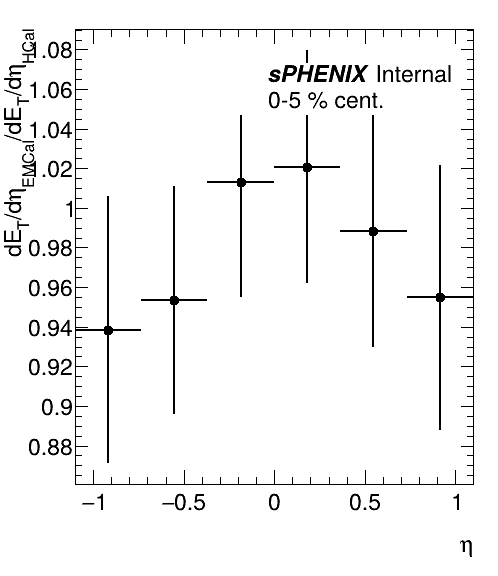
\includegraphics[width=0.32\linewidth]{detdeta/Figures/corr_syst_uncertainties/hcal_emcal_ratio_syst_0-5.png}
    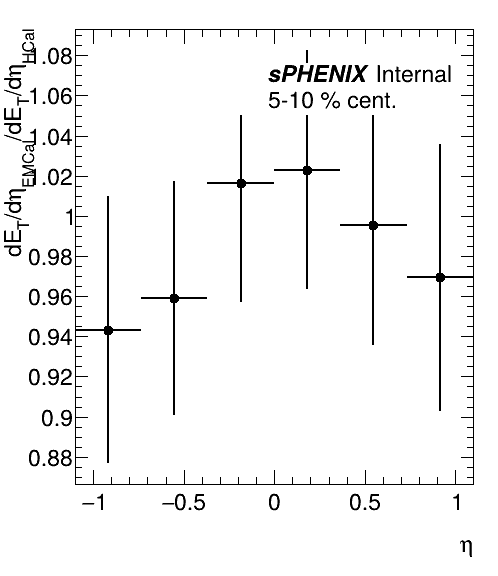
\includegraphics[width=0.32\linewidth]{detdeta/Figures/corr_syst_uncertainties/hcal_emcal_ratio_syst_5-10.png}
    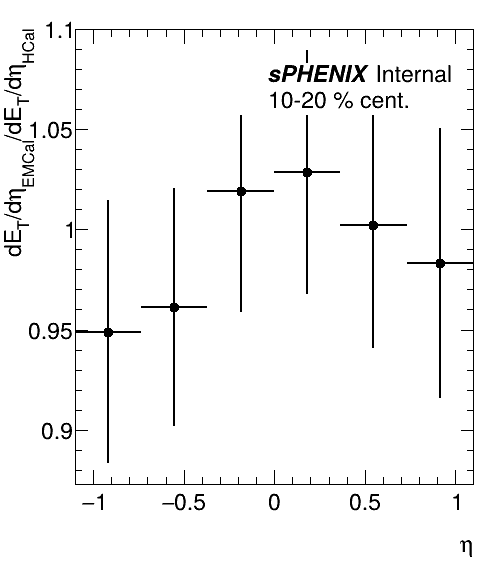
\includegraphics[width=0.32\linewidth]{detdeta/Figures/corr_syst_uncertainties/hcal_emcal_ratio_syst_10-20.png}
    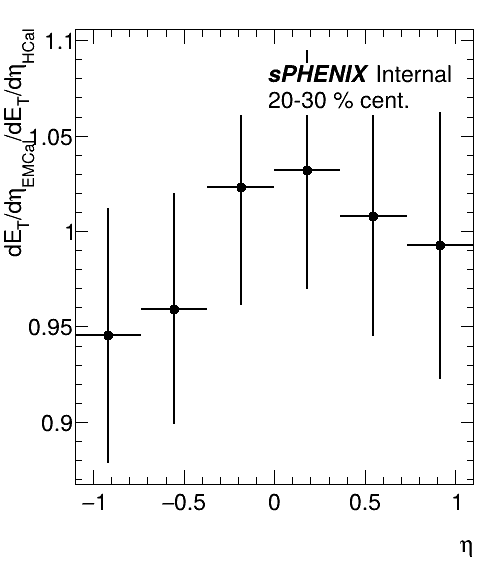
\includegraphics[width=0.32\linewidth]{detdeta/Figures/corr_syst_uncertainties/hcal_emcal_ratio_syst_20-30.png}
    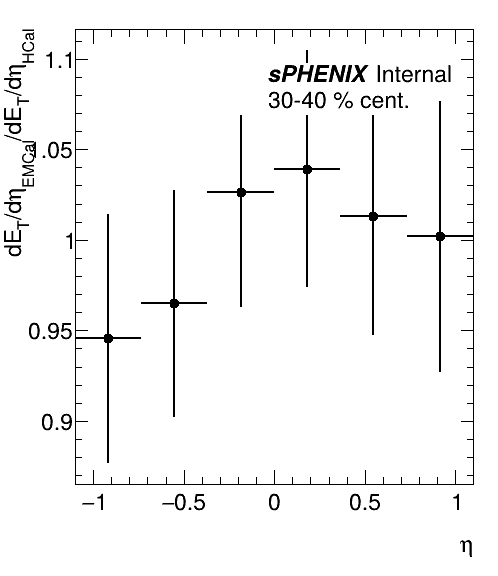
\includegraphics[width=0.32\linewidth]{detdeta/Figures/corr_syst_uncertainties/hcal_emcal_ratio_syst_30-40.png}
    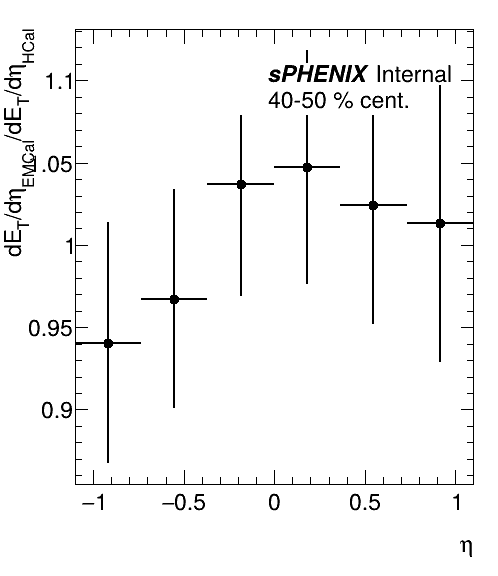
\includegraphics[width=0.32\linewidth]{detdeta/Figures/corr_syst_uncertainties/hcal_emcal_ratio_syst_40-50.png}
    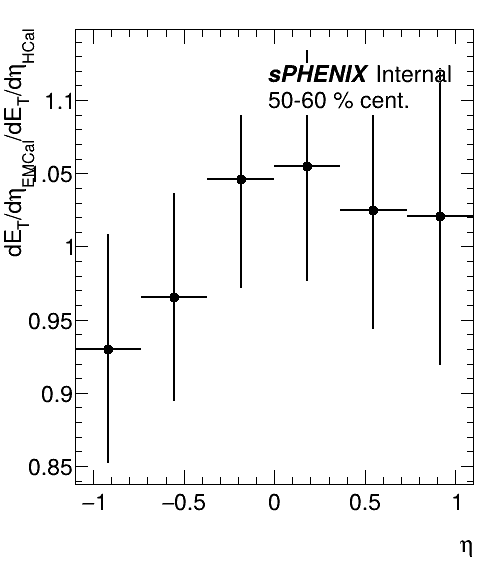
\includegraphics[width=0.32\linewidth]{detdeta/Figures/corr_syst_uncertainties/hcal_emcal_ratio_syst_50-60.png}
    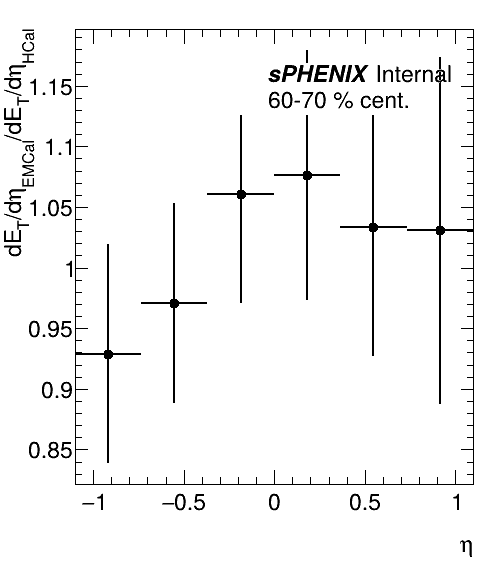
\includegraphics[width=0.32\linewidth]{figures/chapter4/hcal_emcal_ratio_syst_60-70.png}
    \caption{Ratio of the EMCal to HCal \detdeta measurements with full subtraction of correlated measurement uncertainties for each centrality measurement in the analysis. Ratios are shown in central to peripheral events from top to bottom.}
    \label{fig:emcal_hcal_detdeta_ratio}
\end{figure}

\subsubsection{Agreement at Positive and Negative $\eta$}

The level of correlation between the EMCal, HCal and full calorimeter measurements at positive and negative $\eta$ is determined in the same manner as for the test of the agreement between the EMCal and HCal measurements. 
For each measurement, \detdeta is measured in 6 bins across the $\eta$ measurement range $\eta < 1.1$ with 3 bins in each of the positive and negative $\eta$ regions. 
The correlation between each of the 3 pairs of measurements at $|\eta|$ is found using all systematic variations in this analysis for each centrality bin. 
The correlation between the the most forward bins of the measurement ($0.74 < |\eta| < 1.1$) for the full calorimeter measurement for all centrality intervals is shown as a reference in Figure~\ref{fig:calo_eta_covariance}. 
The correlation between positive and negative $\eta$ values of the EMCal-only and HCal-only \detdeta measurements for all centrality intervals are also investigated and included in Appendix~\ref{sec:detdeta_add_syst} as Figures~\ref{fig:emcal_eta_covariance} and \ref{fig:hcal_eta_covariance}. 
The Pearson correlation coefficient is extracted from these correlation plots in the same manner as for the EMCal-HCal correlations. 
For all measurements and $\eta$ ranges, the results are highly correlated in $|\eta|$ as expected from how the uncertainties were devised. 
The correlation coefficients for each of the positive-negative $\eta$ pairs in each calorimeter measurement and each centrality interval are given in Table~\ref{tab:eta_correlation}.

\begin{figure}
    \centering
    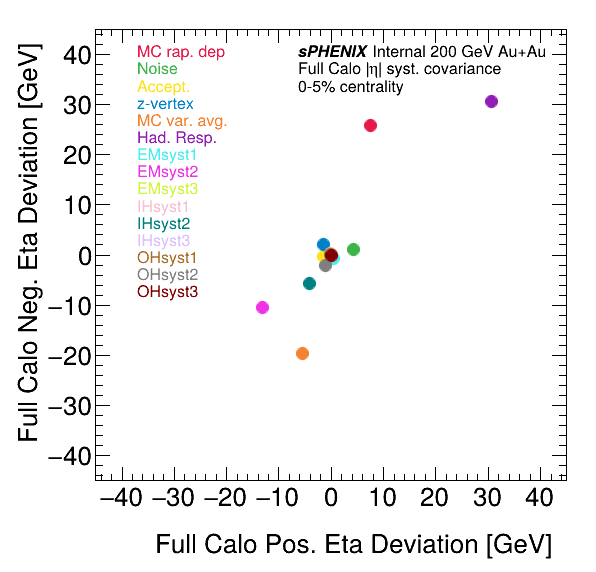
\includegraphics[width=0.32\linewidth] {detdeta/Figures/corr_syst_uncertainties/calo_pos_neg_eta_covariance_0-5.png}
    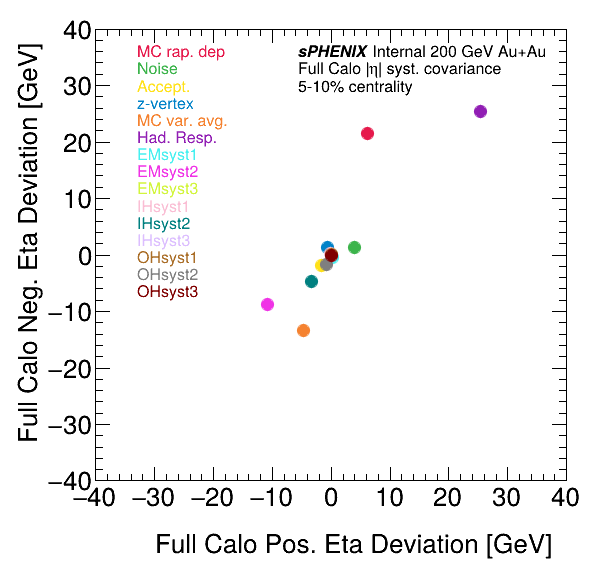
\includegraphics[width=0.32\linewidth]{detdeta/Figures/corr_syst_uncertainties/calo_pos_neg_eta_covariance_5-10.png}
    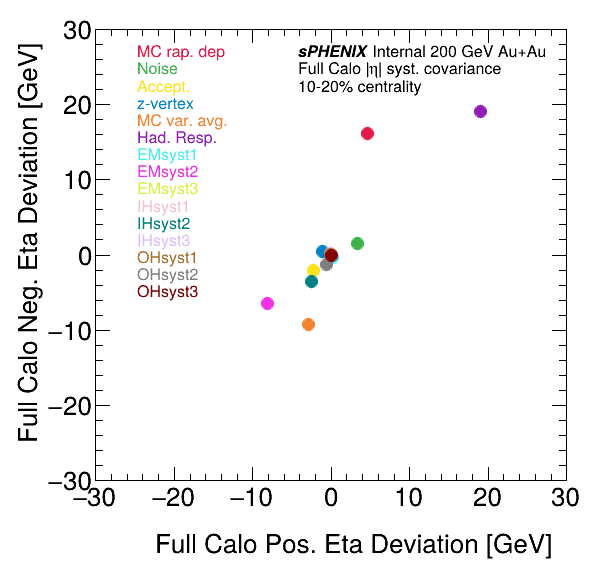
\includegraphics[width=0.32\linewidth]{detdeta/Figures/corr_syst_uncertainties/calo_pos_neg_eta_covariance_10-20.png}
    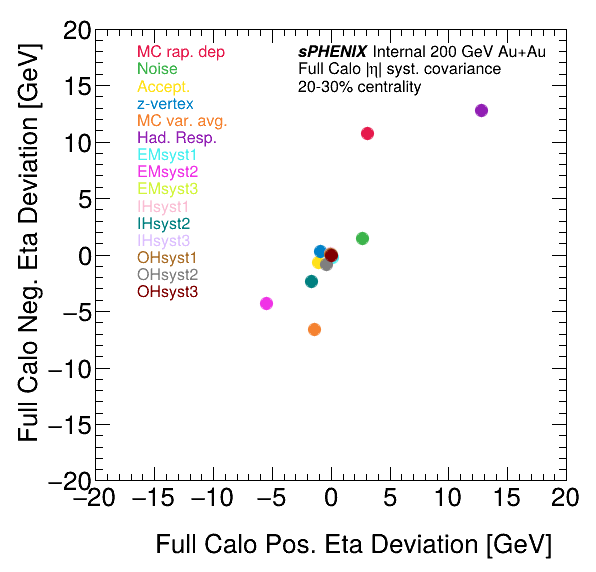
\includegraphics[width=0.32\linewidth]{detdeta/Figures/corr_syst_uncertainties/calo_pos_neg_eta_covariance_20-30.png}
    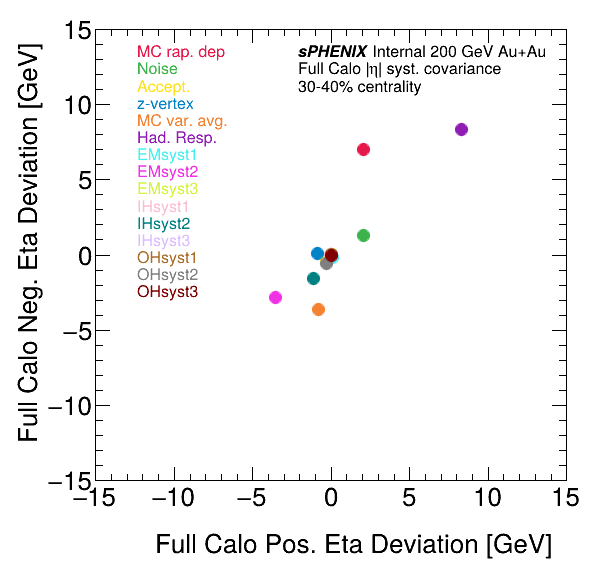
\includegraphics[width=0.32\linewidth]{detdeta/Figures/corr_syst_uncertainties/calo_pos_neg_eta_covariance_30-40.png}
    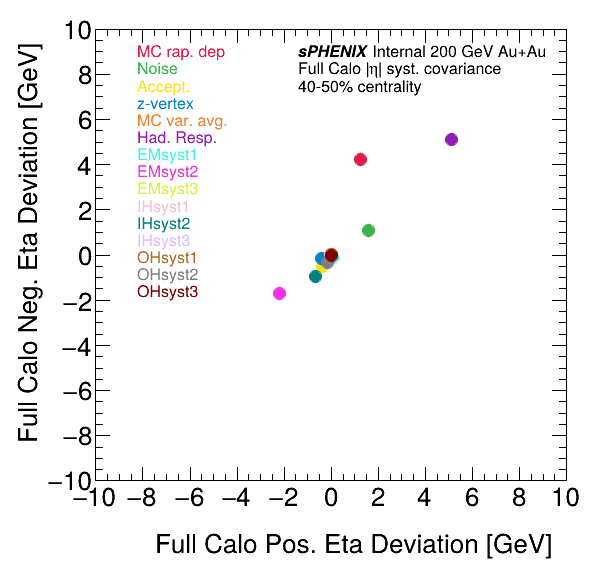
\includegraphics[width=0.32\linewidth]{detdeta/Figures/corr_syst_uncertainties/calo_pos_neg_eta_covariance_40-50.png}
    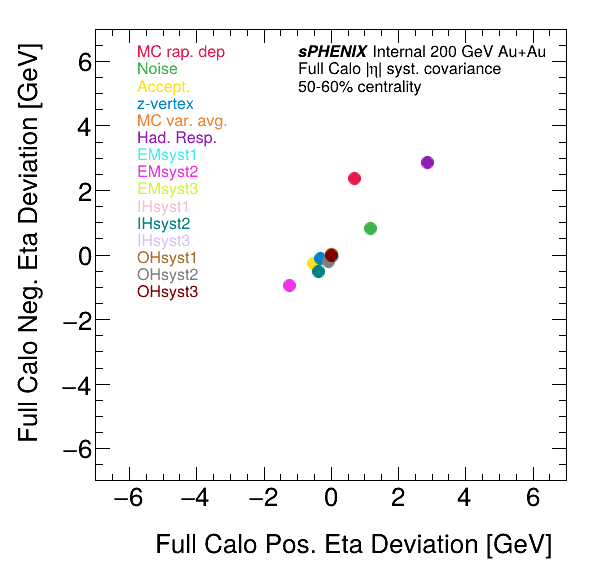
\includegraphics[width=0.32\linewidth]{detdeta/Figures/corr_syst_uncertainties/calo_pos_neg_eta_covariance_50-60.png}
    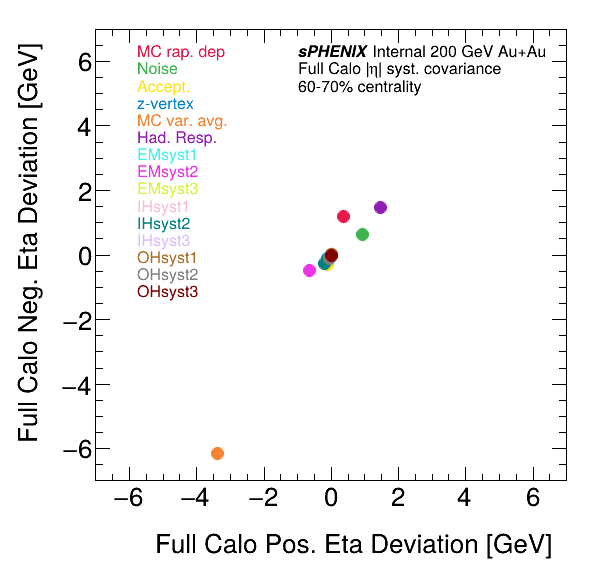
\includegraphics[width=0.32\linewidth]{detdeta/Figures/corr_syst_uncertainties/calo_pos_neg_eta_covariance_60-70.png}
    \caption{Correlation plots for the full calorimeter \detdeta measurements at $0.74 < |\eta| < 1.1$ using each analysis systematic variation for each centrality measurement in the analysis. Uncertainties from all centralities in measurement are shown from central to peripheral events from top to bottom.}
    \label{fig:calo_eta_covariance}
\end{figure}

\begin{table}
    \centering
     \begin{tabular}{c|c|c|c|c|c|c|c|c|c}
    \multirow{2}{*}{Centrality} & \multicolumn{3}{c|}{EMCal} & \multicolumn{3}{c|}{HCal} & \multicolumn{3}{c}{Full Calo} \\
    & $\rho_{\eta_{1}}$ & $\rho_{\eta_{2}}$ & $\rho_{\eta_{3}}$ & $\rho_{\eta_{1}}$ & $\rho_{\eta_{2}}$ & $\rho_{\eta_{3}}$ & $\rho_{\eta_{1}}$ & $\rho_{\eta_{2}}$ & $\rho_{\eta_{3}}$ \\
    \hline
    0-5\%   & 0.99 & 0.98 & 0.92 & 0.99 & 0.96 & 0.84 & 0.99 & 0.97 & 0.85 \\
    5-10\%  & 0.99 & 0.98 & 0.94 & 0.99 & 0.97 & 0.84 & 0.99 & 0.98 & 0.87 \\
    10-20\% & 0.99 & 0.98 & 0.95 & 0.99 & 0.97 & 0.83 & 0.99 & 0.98 & 0.89 \\
    20-30\% & 0.99 & 0.98 & 0.94 & 0.99 & 0.97 & 0.87 & 0.99 & 0.98 & 0.89 \\
    30-40\% & 0.99 & 0.98 & 0.96 & 0.99 & 0.96 & 0.86 & 0.99 & 0.98 & 0.91 \\
    40-50\% & 0.87 & 0.84 & 0.92 & 0.47 & 0.50 & 0.54 & 0.64 & 0.63 & 0.72 \\
    50-60\% & 0.96 & 0.99 & 0.98 & 0.91 & 0.96 & 0.95 & 0.95 & 0.98 & 0.96 \\
    60-70\% & 0.98 & 0.97 & 0.96 & 0.99 & 0.99 & 0.98 & 0.99 & 0.99 & 0.97 \\
    \end{tabular}
    \caption{Correlation coefficient between \detdeta measurements at positive and negative $\eta$ for 3 $|\eta|$ bins of EMCal, HCal and full calorimeter \detdeta measurements for each centrality measurement in the analysis. Here, $\eta_{1}$ refers to $\eta$ bins $0 < |\eta| < 0.36$, $\eta_{2}$ refers to $\eta$ bins $0.36 < |\eta| < 0.74$, and $\eta_{3}$ refers to $\eta$ bins $0.74 < |\eta| < 1.1$.}
    \label{tab:eta_correlation}
\end{table}

The ratio of the \detdeta measurements at positive and negative $\eta$ was found with correct subtraction of correlated uncertainties using the same formula for error propagation as for the EMCal and HCal measurement ratio (Eq.~\ref{eq:emcal_hcal_ratio_uncertainty}). 
Figure~\ref{fig:calo_eta_detdeta_ratio} shows the ratio of the full calorimeter \detdeta measurements at positive and negative $\eta$ for each of the centrality bins in this analysis. 
The ratio of the EMCal and HCal \detdeta measurements at postiive and negative $\eta$ for each centrality bin in the analysis are included in Appendix~\ref{sec:detdeta_add_syst} as Figures~\ref{fig:emcal_eta_detdeta_ratio} and \ref{fig:hcal_eta_detdeta_ratio}.
The measurements at the same $\left|\eta\right|$ are generally consistent across all methods and centralities. 
Small deviations, up to a few percent, are observed at large $\left|\eta\right|$ in the most central intervals and are accounted for within the total estimated uncertainties. 
The ratio agrees with unity for most measurements at the majority of $|\eta|$ bins as can be seen in Figure~\ref{fig:calo_eta_detdeta_ratio} and deviates from unity by at most 1.6 sigma (~4\%) in central collisions at high-eta in the EMCal-only results. 

\begin{figure}
    \centering
    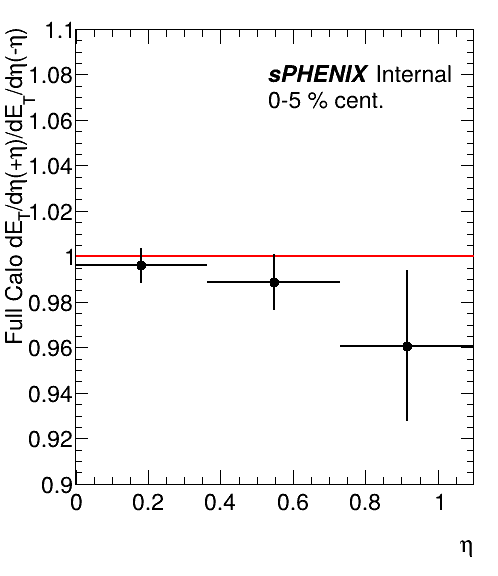
\includegraphics[width=0.32\linewidth]{detdeta/Figures/corr_syst_uncertainties/calo_eta_ratio_syst_0-5.png}
    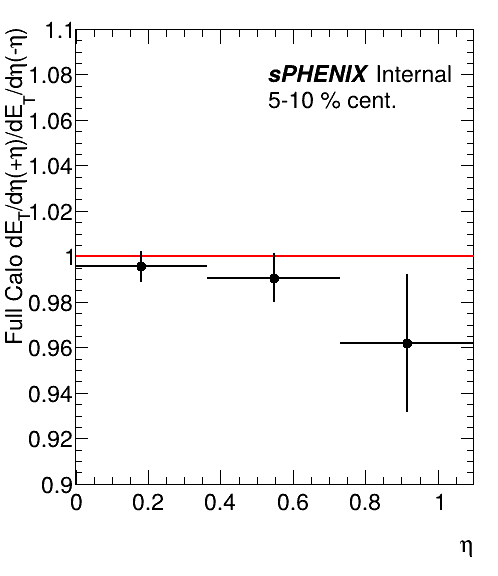
\includegraphics[width=0.32\linewidth]{detdeta/Figures/corr_syst_uncertainties/calo_eta_ratio_syst_5-10.png}
    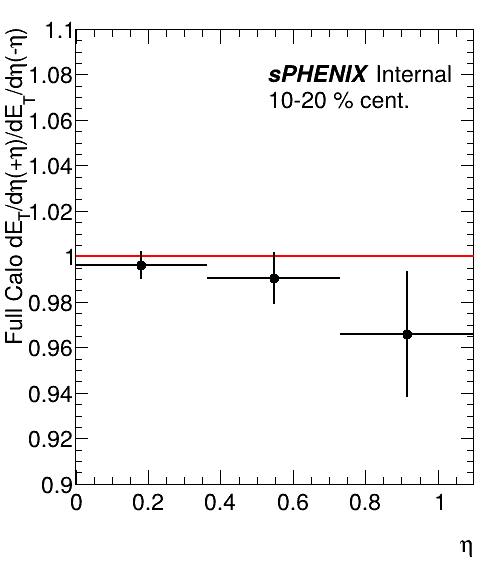
\includegraphics[width=0.32\linewidth]{detdeta/Figures/corr_syst_uncertainties/calo_eta_ratio_syst_10-20.png}
    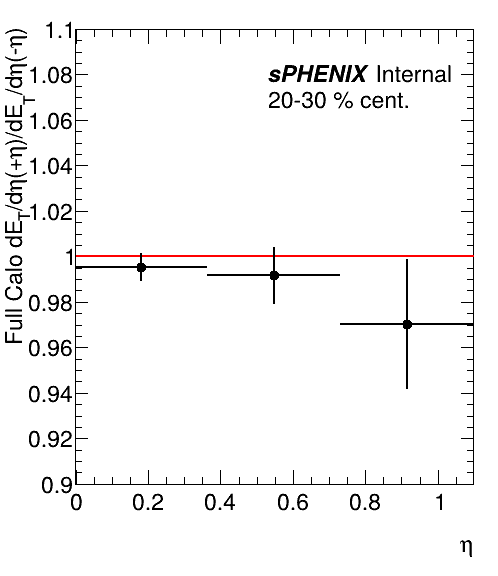
\includegraphics[width=0.32\linewidth]{detdeta/Figures/corr_syst_uncertainties/calo_eta_ratio_syst_20-30.png}
    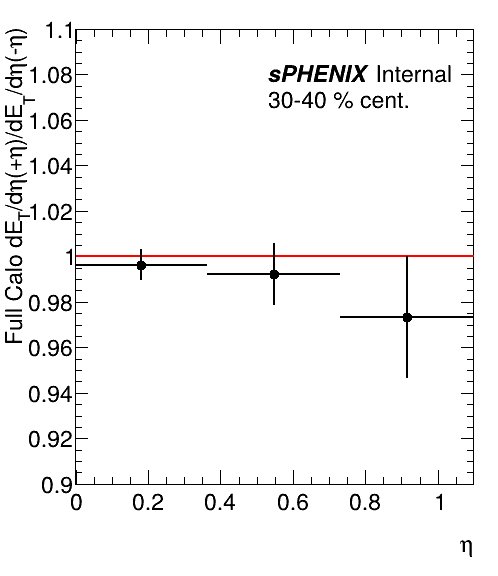
\includegraphics[width=0.32\linewidth]{detdeta/Figures/corr_syst_uncertainties/calo_eta_ratio_syst_30-40.png}
    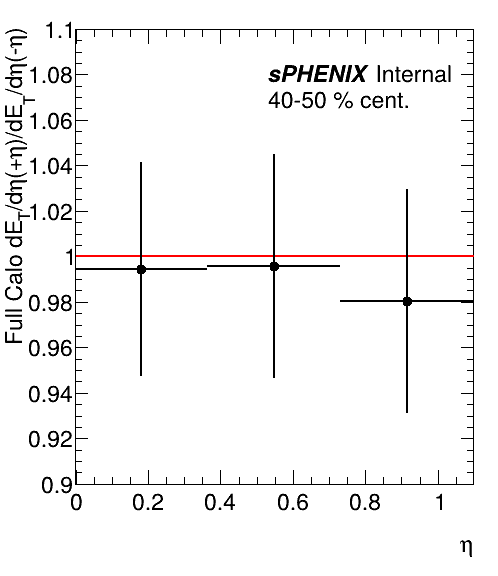
\includegraphics[width=0.32\linewidth]{detdeta/Figures/corr_syst_uncertainties/calo_eta_ratio_syst_40-50.png}
    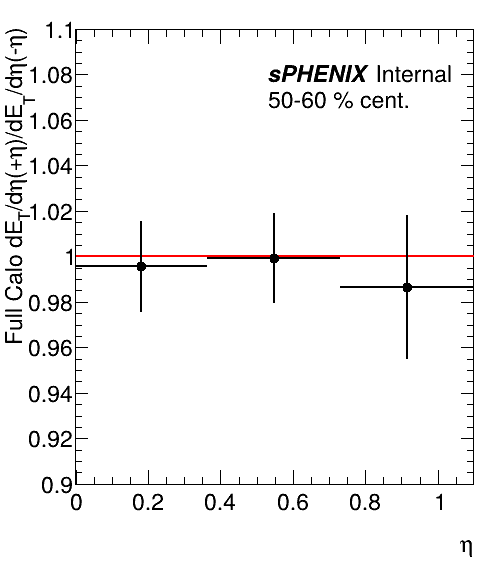
\includegraphics[width=0.32\linewidth]{detdeta/Figures/corr_syst_uncertainties/calo_eta_ratio_syst_50-60.png}
    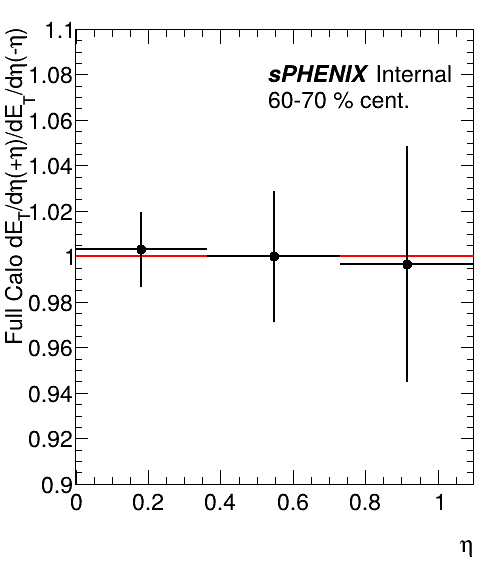
\includegraphics[width=0.32\linewidth]{figures/chapter4/calo_eta_ratio_syst_60-70.png}
    \caption{Correlation plots for the full calorimeter \detdeta measurements at $0.74 < |\eta| < 1.1$ using each analysis systematic variation for each centrality measurement in the analysis. Ratios are shown in central to peripheral events from top to bottom.}
    \label{fig:calo_eta_detdeta_ratio}
\end{figure}